\documentclass[11pt]{article}
\usepackage[margin=1in]{geometry}
\usepackage[T1]{fontenc}
\usepackage{lmodern}
\usepackage{microtype}
\usepackage{natbib}
\usepackage{float}
\usepackage{amssymb}
\usepackage{tikz}
\usetikzlibrary{arrows.meta,positioning,calc,fit}
\usepackage{../shared/smcbvs}
\bibliographystyle{abbrvnat}
\setcitestyle{authoryear,round}
\linespread{1.0}
\renewcommand{\topfraction}{0.95}\renewcommand{\textfraction}{0.05}\renewcommand{\floatpagefraction}{0.75}
\setlength{\emergencystretch}{3em}
\usepackage{url}
\makeatletter\g@addto@macro\UrlBreaks{\do\_\do\-\do\:}\makeatother
\urlstyle{tt}
\DeclareUrlCommand\code{}
\newcommand{\Nc}{N^{\mathrm c}}          % calibration particles
\newcommand{\grid}[1]{\xi_{[#1]}}        % temperatures of the grid
\newcommand{\Lbi}{L_{\mathrm{bi}}}       % burn-in rounds
\newcommand{\Ts}{T_{\mathrm s}}          % number of steps
\newcommand{\Tmax}{T^{\max}}             % step ceiling
\newcommand{\grouprow}[1]{\midrule\multicolumn{6}{@{}l}{\textbf{#1}}\\}
\newcommand{\why}[1]{\par\noindent\textit{Why it matters.} #1\par\smallskip}
\newcommand{\scope}[1]{\par\noindent{\small\textit{Scope.} #1}\par\smallskip}
\newcommand{\asmlist}[1]{\par\smallskip\noindent{\small\textit{Assumptions.} #1}\par\smallskip}
\newcommand{\samplerconds}{two results on the coded sampler (each island realises the frozen run of the theory, and
conditioning on the frozen calibration preserves its identities), proved under their named premises and independently
checked; their final line checks were recorded on 2026-11-17, after the freeze}
% assumptions-section paragraph heads
\newcommand{\SA}[1]{\S\ref{sec:a-#1}}
\makeatletter\defasm{SGR}{SG}\makeatother
\newcommand{\lab}[1]{\textup{(\asmdisp{#1})}}
\newcommand{\SL}{Song and Liang}
\newcommand{\ahead}[3]{\par\smallskip\noindent\textbf{#1} #2. #3\par}
\newcommand{\ev}[1]{\noindent\emph{Evidence.} #1\par}
\newcommand{\ro}[1]{\noindent\emph{Rules out.} #1\par}
\newcommand{\pr}[1]{\noindent\emph{Precedents.} #1\par}
\newcommand{\ds}[1]{\noindent\emph{Our designs.} #1\par}
\newcommand{\tu}[1]{\noindent\emph{A typical user.} #1\par}
\newcommand{\yes}{$\bullet$}\newcommand{\no}{$\circ$}\newcommand{\unc}{?}\newcommand{\na}{--}

\title{SMC-BVS: the model, the sampler, the assumptions and the theorems\\[2pt]
\large Owner-review edition}
\author{SMC-BVS project, Writing Department}
\date{Draft for the owner's review, \today}

\makeatletter\@removefromreset{theorem}{section}\makeatother
\renewcommand{\thetheorem}{\arabic{theorem}}
\begin{document}
\maketitle

% =====================================================================================================
\section{How to read this document}\label{sec:intro}

This edition of the manuscript is written for one reader with two questions: \emph{do the assumptions make sense?} and
\emph{do the theorems look natural and intelligible?} It follows the method from the data to the guarantees, in this
order.
\begin{enumerate}[leftmargin=1.6em,itemsep=1pt]
  \item \emph{The model and the priors} (Section~\ref{sec:method}): what the software assumes and sets, every default with
    the reason for it (Table~\ref{tab:prior}).
  \item \emph{The sampler} (Section~\ref{sec:sampler}): the algorithm as coded, how to read its outputs, which parts the
    theorems cover (Table~\ref{tab:coverage}), and, separately, the parallel engine built for $p=10^6$, which no theorem
    covers.
  \item \emph{The assumptions} (Section~\ref{sec:assumptions}): one table of verdicts (Table~\ref{tab:a-summary}), then one
    entry per assumption with five parts: (a) the statement, (b) its meaning in words, (c) what it rules out, (d) whether it
    is reasonable for real designs, and (e) how it compares with the conditions of \citet{SongLiang2015}, the split-and-merge
    paper.
  \item \emph{The proved results} (Section~\ref{sec:proved}), the main ones first. Each comes in words, then as a formal
    statement, then with a grey status box quoting the project's registry, a paragraph on why it is natural, and a
    comparison with \citet{SongLiang2015}.
  \item \emph{The planned results} (Section~\ref{sec:planned}), each marked \textsf{PLANNED}: nothing there is claimed.
  \item \emph{The statuses} (Section~\ref{sec:statuses}): what changed in the registry since the theory freeze of
    2026-11-17, and the open questions.
\end{enumerate}
The supplement (Appendix~\ref{sec:supp}) holds the minor results, listed first with one line each, and the appendices hold
the notation, the full parameter table with code locations, the conventions in full and the status ledger. The 1M runs and
the benchmarks are reported elsewhere.

\paragraph{The method in one paragraph.} SMC-BVS puts a fixed prior on models and coefficients: a beta-binomial prior on
the model size \citep{ScottBerger2010} and a $g$-prior with a unit ridge, so that the posterior over models is known in
closed form up to its normalising constant, the evidence. Nothing is tuned by the user. The method partitions the
predictors into small blocks of correlated predictors, scores every subset of every block exactly, and combines these
block tables into a \emph{start law}, an approximation of the posterior that can be computed and sampled exactly. A
sequential Monte Carlo sampler, run as four independent \emph{islands}, then moves from the start law to the posterior
along a tempered path that an internal calibration fixes in advance. Two deterministic local searches, one of them from
the mode of the start law, finish the run. The run reports its best model, pooled inclusion probabilities, their median
probability model and an evidence estimate.

\paragraph{What is proved, in one paragraph.} Under the assumptions of Section~\ref{sec:assumptions}: the posterior puts
all but a fraction of order $\rn$ of its mass on the true model (Result~1), and recovers the true conditional law of the
response at that radius, with no lower bound on the coefficients (Result~2). For block and AR designs whose true
coefficients do not cancel, every run that produces output reports exactly the true model, with probability tending to
one, for every seed (Result~3). Without those design conditions, a run rarely certifies a small model that misses a true
predictor (Result~4). The evidence estimate is unbiased on every design (Result~5). The rate $\rn$ cannot be improved
(Result~6). All results are asymptotic in $n$, with $p$ at most polynomial in $n$; this paper contains no simulation study.

\paragraph{What is not claimed.} No theorem covers the parallel engine used at $p=10^6$, more than four islands, or a run
that stops early. Statements about a run's estimates concern the event that its calibration succeeds, or that the run
completes; no lower bound on the probability of that event is claimed, except that under Convention~\as{C2p} every run
produces output. The consistency of the pooled inclusion probabilities and evidence estimate is proved only on designs
without leakage (supplement, Remark~\ref{thm:outputs}).

% =====================================================================================================
\section{Setup and notation}\label{sec:setup}

\paragraph{Notation.} For an integer $k\ge1$, $\set{k}:=\{1,\dots,k\}$. Vectors are columns; $\norm{v}$ and
$\norm{v}_1$ are the Euclidean and $\ell_1$ norms; $I_n$ is the identity and $\one_n$ the vector of ones; $\lmin(\cdot)$
is the smallest eigenvalue of a symmetric matrix; $\abs{S}$ is the size of a set; $a\vee b:=\max(a,b)$; $\ind{E}$ is an
indicator. Logarithms are natural ($\log$) or binary ($\log_2$). A star marks a true value, and the superscript
$\mathrm r$ marks raw, unstandardised data. For a matrix $\Lambda$ and sets $U,V$, $\Lambda_{UV}$ is the sub-matrix with
rows in $U$ and columns in $V$, and $\Lambda_U:=\Lambda_{UU}$. For random variables, $V_n=\OP(a_n)$ means that
$\abs{V_n}/a_n$ is bounded in probability and $V_n=\oP(a_n)$ that it tends to zero in probability; \emph{with probability
tending to one} means that the probability of the event tends to one. For positive sequences, $a_n=O(b_n)$ (or
$a_n\lesssim b_n$, $b_n\gtrsim a_n$) means $a_n\le Cb_n$ for a constant $C$; $a_n=o(b_n)$ means $a_n/b_n\to0$;
$a_n\asymp b_n$ means both $a_n\lesssim b_n$ and $b_n\lesssim a_n$; and $a_n\gg b_n$ means $b_n=o(a_n)$. A quantity is
\emph{fixed} if it does not depend on $n$. All results are asymptotic in $n\to\infty$, along a sequence of problems in
which $p$, the design and the coefficients may change with $n$; every constant introduced in an assumption is fixed.

\paragraph{Data and model.} We observe a response $\yr\in\R^n$ and $\praw$ predictors. The method removes every
predictor that is constant in the sample (its effect is absorbed by the intercept); $\Xr$ is the $n\times p$ matrix of
the $p$ retained predictors, and from here on $p$ always means this number. The data follow a Gaussian linear model with
an intercept,
\begin{equation}\label{eq:model}
  \yr=\alpha^*\one_n+\Xr\bstar+\varepsilon,\qquad \varepsilon\sim\Normal_n(0,\sigs^2I_n),
\end{equation}
with $\sigs^2>0$ and $\varepsilon$ independent of $\Xr$. A \emph{model} is a set $S\subseteq\set{p}$; the \emph{true
model} is $\Sz:=\{j:\beta^*_j\neq0\}$, of size $\sz$. Its members are the \emph{true predictors}, the others the
\emph{null predictors}. In a \emph{fixed design} $\Xr$ is deterministic and probability refers to the noise. In a
\emph{random Gaussian design} the rows of $\Xr$ are i.i.d.\ $\Normal_p(m_n,\Sig)$ and probability refers to the joint law
of design and noise; $W=(W_1,\dots,W_p)\sim\Normal_p(0,\Sig)$ denotes a centred copy of one row, with sub-vectors $W_S$.

\paragraph{Standardisation.} The method centres and scales every predictor and the response. With
$P^\perp_{\one}:=I_n-n^{-1}\one\one^\top$ and $D$ the diagonal matrix of the column sample standard deviations (divisor
$n-1$),
\begin{equation}\label{eq:standardise}
  X:=P^\perp_{\one}\Xr D^{-1},\qquad y:=P^\perp_{\one}\yr/s_y,\qquad s_y^2:=\norm{P^\perp_{\one}\yr}^2/(n-1),
\end{equation}
so every column $x_j$ of $X$ has mean zero and $\norm{x_j}^2=n-1$, and $y^\top y=n-1$. In these terms
$P^\perp_{\one}\yr=X\tstar+P^\perp_{\one}\varepsilon$, with the \emph{standardised coefficients} $\tstar:=D\bstar$ (same
support $\Sz$), the \emph{mean signal} $\mu:=X\tstar$, and $\tmin:=\min_{j\in\Sz}\abs{\theta^*_j}$. For a model $S$, $X_S$
holds its columns, $G_S:=X_S^\top X_S$ is their Gram matrix, $\Rhat_S:=G_S/(n-1)$ their sample correlation matrix,
$\hat r_{jl}$ the sample correlation of predictors $j$ and $l$, $P_S$ the projection onto their span ($P_\emptyset:=0$),
and $z_S:=X_S^\top y$.

% =====================================================================================================
\section{The model and the priors}\label{sec:method}\label{sec:prior}

This section says what the method assumes about the data and what prior it puts on models and coefficients. Every
choice is fixed by the software; the user sets nothing. Table~\ref{tab:prior} lists each choice with its default and
the reason for it; Appendix~\ref{app:params} gives the code location of every constant.

\paragraph{Working model.} Given a model $S$, coefficients $\theta_S\in\R^{\abs{S}}$ and a variance $\sigma^2>0$, the
method fits $y\mid S,\theta_S,\sigma^2\sim\Normal_n(X_S\theta_S,\sigma^2I_n)$ to the standardised data of
Section~\ref{sec:setup}. Here $\theta_S$ and $\sigma^2$ are working parameters; the intercept is removed by centring.
The theorems are proved under the true model~\eqref{eq:model}, not under this working model.

\paragraph{Model space and model prior.} The method considers every model with at most $K$ predictors,
\begin{equation}\label{eq:space}
  \Om:=\{S\subseteq\set{p}:\abs{S}\le K\},\qquad K:=\min\big(p,\lfloor n/2\rfloor\big),
\end{equation}
and gives a model a prior probability that depends only on its size:
\begin{equation}\label{eq:modelprior}
  \text{prior of }S=\frac{w(\abs{S})}{\bar w_K},\qquad w(k):=\frac{1}{2\binom{2p-1}{k}},\qquad
  \bar w_K:=\sum_{k=0}^{K}\binom{p}{k}w(k).
\end{equation}
This is the beta-binomial prior $\BB(1,p)$ \citep{ScottBerger2010} restricted to $\Om$: a probability $q$ is drawn from
$\BetaDist(1,p)$, and given $q$ each predictor enters independently with probability $q$. Its mean model size is about
one. Adding a predictor to a model of size $k$ multiplies the prior by $(k+1)/(2p-1-k)$, a cost of about
$\log\{2p/(k+1)\}$ in log prior odds. For example, with $p=3$ and $n\ge6$ the empty model has prior probability
$\tfrac12$, each one-predictor model $\tfrac1{10}$, and each larger model $\tfrac1{20}$.

\paragraph{Coefficients and noise variance.} Given $S$ and $\sigma^2$, the coefficients have a $g$-prior
\citep{Zellner1986} with $g=n$ and a unit ridge, and the variance an inverse-gamma prior:
\begin{equation}\label{eq:slab}
  \theta_S\mid S,\sigma^2\sim\Normal\big(0,\;n\sigma^2(G_S+I)^{-1}\big),\qquad \sigma^2\sim\IG(a_0,b_0),\quad a_0=b_0=0.01 .
\end{equation}

\begin{table}[ht]
\centering\small
\setlength{\tabcolsep}{4pt}
\caption{The model and the priors: every choice, its default, and why. Nothing here is tuned by the user.}\label{tab:prior}
\begin{tabular}{@{}>{\raggedright\arraybackslash}p{0.2\linewidth}>{\raggedright\arraybackslash}p{0.24\linewidth}>{\raggedright\arraybackslash}p{0.5\linewidth}@{}}
\toprule
Choice & Default & Why \\
\midrule
likelihood & Gaussian linear model with an intercept on the raw scale; the method centres and scales the data and
scores the centred model, with no intercept parameter &
the standard model for variable selection; standardising makes the posterior unchanged when the response is shifted or
rescaled, and puts every predictor on one scale, so one prior fits all. \\
model-size prior & $\BB(1,p)$: $w(k)=\tfrac12/\binom{2p-1}{k}$ &
corrects for multiplicity \citep{ScottBerger2010}: each extra predictor costs about $\log(2p)$ in log prior odds,
the order needed to keep $p$ null predictors out; it has no parameter to tune; its mean model size is about one. \\
size cap & $K=\min(p,\lfloor n/2\rfloor)$ &
a model with more predictors than about half the observations cannot be estimated reliably; the cap keeps every model's
fit well posed and bounds the model space. \\
coefficient prior & $g$-prior, $g=n$ &
a unit-information prior: worth about one observation; it costs each extra predictor about $\tfrac12\log n$ in the
marginal likelihood, a BIC-like penalty. \\
ridge & unit ridge, $G_S+I$ &
keeps the prior proper when the columns of a model are collinear, which happens when $p>n$; it is negligible when
$G_S$ is of order $n$. \\
noise-variance prior & $\IG(0.01,0.01)$ &
proper, and close to the usual non-informative $1/\sigma^2$; with $n$ observations its parameters change the posterior
very little. \\
\bottomrule
\end{tabular}
\end{table}

\subsection{The posterior, in closed form}\label{sec:posterior}

Integrating $\theta_S$ and $\sigma^2$ out gives the marginal likelihood of each model,
\begin{equation}\label{eq:marglik}
  m(S)=C_n\Big(\frac{\det H_S}{\det(G_S+I)}\Big)^{-1/2}(2b_0+\SSq_S)^{-\nu},\quad
  H_S:=(n+1)G_S+I,\ \ \SSq_S:=y^\top y-n\,z_S^\top H_S^{-1}z_S,
\end{equation}
with $\nu:=a_0+n/2$ and $C_n:=(2b_0)^{a_0}\Gamma(a_0+n/2)/\{\pi^{n/2}\Gamma(a_0)\}$ (here $\pi=3.14\ldots$).
$\SSq_S$ is a shrunken residual sum of squares. The determinant ratio is a penalty for size (an Occam factor): in a
well-conditioned model it multiplies $m(S)$ by about $(n+1)^{-1/2}$ for each extra predictor. The \emph{log score} of a
model and the \emph{posterior over models} are
\begin{equation}\label{eq:posterior}
  F(S):=\log\{w(\abs{S})/\bar w_K\}+\log m(S),\qquad \pis{S}=\frac{e^{F(S)}}{Z},\qquad Z:=\sum_{S'\in\Om}e^{F(S')} .
\end{equation}
The normalising constant $Z$ is the \emph{evidence}. So the posterior is known exactly up to one number; the whole
difficulty is that $\Om$ is too large to sum over, which is what the sampler of Section~\ref{sec:sampler} is for.

The posterior is summarised by four quantities. The \emph{inclusion probability} of predictor $j$ is
$\PIP_j:=\sum_{S\ni j}\pis{S}$; the \emph{highest posterior model} is $\HPM:=\argmax_S\pis{S}$; the \emph{median
probability model} is $\MPM:=\{j:\PIP_j>1/2\}$ \citep{BarbieriBerger2004}; and the \emph{posterior miss} is
$1-\pis{\Sz}$, the posterior mass outside the true model.

\begin{lemma}[The posterior miss controls the summaries]\label{lem:summaries}
For every data set, $\max_{j\in\set{p}}\abs{\PIP_j-\ind{j\in\Sz}}\le1-\pis{\Sz}$. If $\pis{\Sz}>1/2$, then
$\HPM=\MPM=\Sz$.
\end{lemma}

The proof is two lines: every model that misses a true predictor, or contains a null one, differs from $\Sz$. So a
theorem that makes the posterior miss small makes every summary right at once.

\paragraph{Compared with \SL.} The two priors are close in kind. \emph{Model prior:} theirs lets each predictor enter
independently with probability $\lambda_n=r_n/P_n$, where $P_n$ is their number of predictors (our $p$), and caps the model size at $\bar r_n$ (their (6), p.~951); both $r_n$
and $\bar r_n$ are chosen by the user, and their Theorems~1--3 need $\lambda_n\to0$ (their (13), p.~952). Ours mixes over the inclusion probability
(beta-binomial), which costs each predictor about $\log p$ in log prior odds, as theirs does for their usual choices of $r_n$, with nothing to choose, and fixes the cap at
$\lfloor n/2\rfloor$. \emph{Coefficients:} theirs is $\Normal(0,\sigma^2V_\xi)$ with a user-chosen $V_\xi$ (p.~951); in
their numerical work $V_\xi^{-1}=(X_\xi^\top X_\xi+\tau I)/n$ with $\tau=0.01$ (p.~959). Ours is exactly this form with
$\tau=1$. \emph{Noise:} both use an inverse-gamma prior; theirs takes $a_0=b_0=1$ in their numerical work (pp.~959--960), ours
$0.01$.

% =====================================================================================================
\section{The sampler}\label{sec:sampler}

This section describes the algorithm as the software (an R package with a C++ core) implements it in its default
configuration, and how to read what it reports. The user supplies the data, a random seed and a computing allocation;
everything else is a numerical constant or a stated function of $(n,p)$ (Appendix~\ref{app:params} lists every one, with its code location). The last two
subsections say which parts the theorems cover, and describe separately the parallel engine built for $p=10^6$, which no
theorem covers.

\subsection{Why sequential Monte Carlo, and why this start law}\label{sec:intuition}

The posterior is known up to one constant, so the difficulty is to find where its mass is in an enormous, rugged model
space. It is rugged for two reasons: correlated predictors create near-ties between models that swap a true predictor for
its proxy, and a predictor that is useless once the true ones are in can look useful on its own, because it \emph{leaks}
part of their signal. Sequential Monte Carlo starts many models (\emph{particles}) from an easy distribution close to the
target and moves them to the target in small steps, copying the particles the next distribution favours and spreading
them with Markov moves. The \emph{start law} is that easy distribution: it scores every subset of each block of correlated
predictors exactly, so it resolves a true predictor against its proxies, and it can be sampled exactly. What it gets wrong
is leakage across blocks. The local search from its mode undoes that, deleting the spurious predictors one per move; it
uses no random numbers, so it gives a second route to the true model that does not depend on how well the particles
mixed.

\begin{example}[Leakage, with six predictors]\label{ex:leak}
Take $n=100$, true model $\{1,3\}$ with both coefficients $1$, and unit noise. Predictor $2$ is a proxy of $1$
(correlation $0.93$); $4$ is moderately correlated with $3$ ($0.69$); $5$ is correlated with $1$ ($0.63$); and $6$ is a
proxy of $5$ ($0.89$). With blocks $\{1,2\}$, $\{3,4\}$, $\{5,6\}$, the five models with the largest posterior mass are:

\smallskip
\centerline{\small
\begin{tabular}{@{}lccccc@{}}
\toprule
model & $\{1,3,5\}$ & $\{1,3\}$ & $\{1,3,6\}$ & $\{1,3,4\}$ & $\{1,2,3\}$ \\
\midrule
start law $\pi_0$ & $\mathbf{0.517}$ & $0.198$ & $0.067$ & $0.012$ & $0.008$ \\
posterior $\pi(\cdot\mid y)$ & $0.042$ & $\mathbf{0.688}$ & $0.118$ & $0.051$ & $0.037$ \\
\bottomrule
\end{tabular}}
\smallskip

Within its own block, predictor $5$ explains much of $y$ because it carries part of predictor $1$'s signal, and the
start law cannot see that predictor $1$, in another block, already explains it: predictor $5$ leaks, and the start mode is
$\{1,3,5\}$. The proxy $2$, in predictor $1$'s own block, is handled correctly. The posterior puts $0.69$ on $\{1,3\}$, and
the local search from the start mode makes one move, deleting $5$, and stops at $\{1,3\}$, which has no improving
neighbour. The example only illustrates the mechanism. Result~3 shows that, asymptotically and under its assumptions, this
is what happens in general: the start mode contains the true model and possibly some predictors that enter it wrongly
(here predictor~$5$), all members of a small \emph{leakage set} (Section~\ref{sec:a-rm}), and the search deletes them. (Computed with an independent re-implementation of the coded score,
start law and search on this data set; with six predictors the software itself would enumerate all $64$ models.)
\end{example}

\subsection{The algorithm, step by step}\label{sec:algorithm}

A run has seven stages (Figure~\ref{fig:pipeline}). A \emph{step} is one move of the sampler from one temperature to the
next (the temperatures $\xi$ are defined at stages 4 and 5; $\pi_1$ is the posterior).

\begin{figure}[ht]
\centering
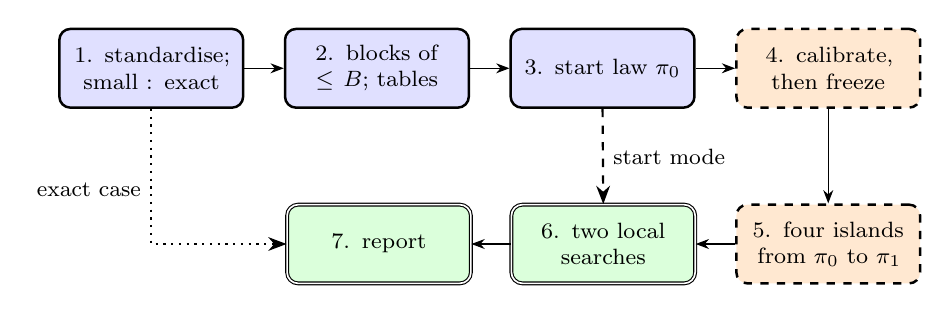
\begin{tikzpicture}[node distance=5mm, every node/.style={font=\footnotesize},
  box/.style={draw, rounded corners, align=center, minimum height=10mm, text width=21mm},
  exact/.style={box, fill=blue!12, line width=0.9pt}, stoch/.style={box, fill=orange!18, dashed, line width=0.9pt},
  det/.style={box, fill=green!14, double}]
\node[exact] (pre) {1. standardise;\\ small $\Om$: exact};
\node[exact, right=of pre] (blk) {2. blocks of\\ $\le B$; tables};
\node[exact, right=of blk] (start) {3. start law $\pi_0$};
\node[stoch, right=of start] (cal) {4. calibrate,\\ then freeze};
\node[stoch, below=12mm of cal] (smc) {5. four islands\\ from $\pi_0$ to $\pi_1$};
\node[det, left=of smc] (ls) {6. two local\\ searches};
\node[det, left=of ls] (out) {7. report};
\draw[-{Stealth}] (pre)--(blk); \draw[-{Stealth}] (blk)--(start); \draw[-{Stealth}] (start)--(cal);
\draw[-{Stealth}] (cal)--(smc); \draw[-{Stealth}] (smc)--(ls); \draw[-{Stealth}] (ls)--(out);
\draw[-{Stealth}, dashed, thick] (start.south) -- node[right, pos=0.5]{start mode $\tSz$} (ls.north);
\draw[-{Stealth}, dotted, thick] (pre.south) |- node[left, pos=0.3]{exact case} (out.west);
\end{tikzpicture}
\caption{The stages of a run. Exact computations: solid boxes (1--3). Random: dashed boxes (4--5). Deterministic given
their inputs: double boxes (6--7). When $\Om$ is small the run goes from stage~1 straight to the report (dotted). The
second local search starts from the start mode and does not depend on the particles (dashed arrow).}
\label{fig:pipeline}
\end{figure}

\paragraph{Stage 1: inputs, the exact case and the check before the run.} Invalid inputs stop the run with no model; a constant response, or no retained predictor, stops it with the empty
model and no estimates. If the model space is small, at most $(5\Nc_0+4N_0)\,p$ models with $N_0:=\max(2500,n,p)$ and
$\Nc_0:=\lceil512N_0/2500\rceil$ (Appendix~\ref{app:params}), the method scores every model and computes everything
exactly. Otherwise it estimates the memory the run will need and the worst-case time of the local search from the start
mode, and stops with status \texttt{resource\_limit} if the
estimate exceeds the allocation (8\,GiB and 24 hours by default).

\paragraph{Stage 2: blocks and block tables.} The method partitions the predictors into blocks $C_1,\dots,C_J$ of at most
$B:=\min(\lfloor\sqrt n\rfloor,\lfloor\sqrt p\rfloor,16)$ predictors, by complete-linkage clustering on $1-\abs{\hat r_{jl}}$,
cutting the tree top-down until every cluster fits and packing whole clusters into blocks in leaf order. The partition is a
deterministic function of $X$, and correlated predictors tend to share a block. Within each block it scores every subset
$U$ with $\abs{U}\le K$ and stores the \emph{block table} $h_k(U):=m(U)/m(\emptyset)$, with $h_k(\emptyset)=1$; a block has
at most $2^{16}$ subsets. It also builds a \emph{neighbour graph} of correlated predictors for the swap moves
(Appendix~\ref{app:params}).

\paragraph{Stage 3: the start law and the start mode.} The start law multiplies the size prior by the block tables,
\begin{equation}\label{eq:startlaw}
  \pi_0(S)=\frac{\gamma_0(S)}{\bar Z_0},\qquad \gamma_0(S):=\frac{w(\abs{S})}{\bar w_K}\prod_{k=1}^J h_k(S\cap C_k),\qquad
  \bar Z_0:=\sum_{S\in\Om}\gamma_0(S):
\end{equation}
the posterior one would have if the marginal likelihood, relative to the empty model, split into independent block
contributions. It sees every interaction within a block and none between blocks. A recursion over model sizes, combining
the blocks one at a time, computes $\bar Z_0$ exactly and gives an exact sampler for $\pi_0$ (draw the total size, then
the size of each block, from the last block to the first, then a subset of each block). The \emph{start mode} $\tSz$ is a maximiser of $\pi_0$,
computed by the same recursion with maxima: the smallest size among the maximisers, then the lexicographically smallest
set. The posterior and the start law differ by the \emph{discrepancy}
$\Delta(S):=\log\{m(S)/m(\emptyset)\}-\sum_k\log h_k(S\cap C_k)$, the part of the log marginal likelihood that comes from
interactions between blocks: $\gamma_0(S)e^{\Delta(S)}=e^{F(S)}/m(\emptyset)$.

\paragraph{Stages 4 and 5: the sampler.} The sampler moves through the distributions
\begin{equation}\label{eq:path}
  \pi_\xi\ \propto\ \gamma_0\,e^{\xi\Delta},\qquad 0\le\xi\le1,
\end{equation}
from the start law ($\xi=0$) to the posterior ($\xi=1$), along a grid of temperatures $0=\grid0<\dots<\grid{\Ts}=1$ fixed
by the calibration. An island of $N$ particles starts from $N$ independent draws from $\pi_0$. At each step $t$ it
\begin{enumerate}[label=(\alph*),leftmargin=2em,itemsep=0pt,topsep=2pt]
  \item \emph{reweights} particle $v$ by $\omega^{(t)}_v:=\exp\{(\grid t-\grid{t-1})\Delta(S_v)\}$;
  \item \emph{resamples} the particles multinomially, in proportion to these weights;
  \item \emph{moves} every particle by one round of Markov moves that leave $\pi_{\grid t}$ invariant.
\end{enumerate}
A round is an inclusion update (Gibbs) for each predictor, one uniform swap, $B$ swaps along the neighbour graph, and one
independence move that proposes a fresh draw from $\pi_0$. At $\xi=1$ it runs $\Lbi:=\max(4,\lceil\log_2(n+1)\rceil)$ burn-in rounds
and four measured rounds. The island's inclusion-probability estimate $\PIPhat_{r,j}$ averages, over particles and measured
rounds, the conditional inclusion probability of the Gibbs update rather than the 0/1 indicator; its evidence estimate is
$\Zhat_r:=m(\emptyset)\,\bar Z_0\prod_{t=1}^{\Ts}\{N^{-1}\sum_v\omega^{(t)}_v\}$, the exact normaliser of the start law times
the product of the average reweighting factors.

The \emph{calibration} (stage 4) chooses the grid and the effort before the final run, from one pilot island and a few
rounds of four short diagnostic islands; the grid is chosen so that each step keeps at least $90\%$ effective sample
size, computed on a set of candidate models. The calibration starts at
tier $i=0$ and moves at most once to tier $i=1$, which multiplies all particle numbers by four, when one of its
diagnostics fires (Appendix~\ref{sec:supp-cal} gives the full procedure). Three facts are all that the results use: the calibration's outcome is a function of the data and of its own
random numbers; it is \emph{frozen} before the final run draws any random number; and it \emph{succeeds} when it freezes a
grid, by its main construction or a fallback (otherwise the run stops without estimates). The \emph{final run} (stage 5)
consists of four independent \emph{islands} of $N_i=4^iN_0$ particles at the frozen tier $i$, on the frozen grid, each with
its own random stream.

\paragraph{Stage 6: the local searches.} Two models are \emph{neighbours} if one comes from the other by deleting a
predictor, adding one (while the size is below $K$), or swapping a member for a non-member. A local search scans every
neighbour of the current model and moves to the best one (ties broken lexicographically) if its log score is strictly
higher, for at most a capped number of moves. If a scan finds no strictly better neighbour, the search stops and its end
point is \emph{certified} (a local optimum). If it uses up its move cap first, it scans once more: the end point is
certified if that scan finds no improvement, and uncertified otherwise. Two searches run after the islands: from the best model found so far, with move cap
$\ell_n:=\lceil\log_2(n+p+1)\rceil$; and from the start mode $\tSz$, with move cap $\ell_n+\abs{\tSz}$.

\subsection{What a run reports}\label{sec:outputs-method}

A run ends in one of three ways: \emph{exact} ($\Om$ was enumerated), \emph{completed} (the sampler ran to the end; a
\emph{completed run}), or \emph{stopped} (for example by the resource guard, which stops a run whose time or memory would
exceed its allocation). The first two \emph{produce output}. A stopped run reports no estimates; any partial output is
flagged incomplete, and no result covers it. The method records every model
it scores; the \emph{reported model} $\Shat$ is the best of them by log score (exact ties to the smaller model, then
lexicographically). It is \emph{certified} when the method enumerated $\Om$, or when $\Shat$ ends a local search whose last
scan found no strict improvement. An exact run reports $\Shat$, every $\PIP_j$, the median probability model and $\log Z$.
A completed run pools its islands with equal weights,
\begin{equation}\label{eq:pool}
  \PIPhat_j:=\frac14\sum_{r=1}^4\PIPhat_{r,j},\qquad \Zhat:=\frac14\sum_{r=1}^4\Zhat_r,
\end{equation}
and reports $\Shat$, the $\PIPhat_j$, $\MPMhat:=\{j:\PIPhat_j>1/2\}$, $\log\Zhat$ with the lower bound
$\log(0.05\,\Zhat)$, a flag saying whether $\Shat$ is certified, and the list $\mathcal T$ of the best (at most $40p+1$)
models it scored, with their log scores. Islands are not weighted by their evidence estimates. Diagnostics never change an
output (Appendix~\ref{app:params}).

\paragraph{How to read the outputs.} Each output is an estimate of one posterior summary of
Section~\ref{sec:posterior}, and the theorems of Section~\ref{sec:proved} say when it can be trusted.
\begin{itemize}[leftmargin=1.5em,itemsep=1pt]
  \item \emph{The reported model $\Shat$} is the run's estimate of the highest posterior model. It is the best model the
    run scored, so it equals $\HPM$ when the run has scored $\HPM$; when $\Shat$ is certified, no single addition,
    deletion or swap improves it. Result~3 says when $\Shat=\Sz$; Result~4 says when a certified small $\Shat$ cannot miss
    a true predictor.
  \item \emph{The inclusion probabilities $\PIPhat_j$} estimate $\PIP_j$. Each island averages, over its particles and
    four measured rounds, the probability that the Gibbs update would include $j$ (a Rao--Blackwellised average, less
    noisy than counting inclusions); the four islands are averaged with equal weights. A value near $1$ or $0$ means near-certain
    inclusion or exclusion.
  \item \emph{The median probability model $\MPMhat$} is the set of predictors with $\PIPhat_j>1/2$; it estimates $\MPM$,
    the model that is optimal for prediction under conditions of \citet{BarbieriBerger2004}.
  \item \emph{The evidence $\log\Zhat$} estimates $\log Z$, the marginal probability of the data under the whole prior;
    it is what one compares across priors or data sets. Given the calibration, $\Zhat$ is unbiased for $Z$
    (Result~5), so, by Markov's inequality, the probability that the run completes and still reports a lower bound
    $\log(0.05\,\Zhat)$ above $\log Z$ is at most $0.05$.
  \item \emph{The returned list $\mathcal T$} holds the best models scored, with their exact log scores; renormalising
    the posterior to it gives a second set of estimates (supplement, Corollary~\ref{cor:list}).
\end{itemize}
At moderate $n$ these outputs describe a posterior spread over the true model and many one-predictor extensions of it,
not a point mass: in single synthetic draws at $n=200$ the one-predictor extensions together weighed about as much as the
true model itself (Remark~\ref{rem:moderate-n}; Result~6 explains why).

\subsection{What the theorems cover, and what is engineering}\label{sec:coverage}

The theorems are about the method as coded, but they use only a few properties of each stage. Table~\ref{tab:coverage}
says, stage by stage, what a theorem relies on and what is engineering: a choice that makes the software fast or
robust, that no theorem depends on, and that could be changed without touching any statement.

\begin{table}[ht]
\centering\small
\setlength{\tabcolsep}{4pt}
\caption{Which parts of the method the theorems cover. ``Engineering'' means that no theorem depends on the choice.}\label{tab:coverage}
\begin{tabular}{@{}>{\raggedright\arraybackslash}p{0.2\linewidth}>{\raggedright\arraybackslash}p{0.42\linewidth}>{\raggedright\arraybackslash}p{0.32\linewidth}@{}}
\toprule
Part & What the theorems use & Engineering only \\
\midrule
model, priors, posterior & everything: Results 1, 2 and 6 are about this posterior & --- \\
stage 1 & the exact case (Results 3, 4 and Corollary~\ref{cor:list} include it) & the check before the run and the
resource guard (the theorems assume enough memory and time, Convention~\as{C2p}) \\
stage 2, blocks & blocks of at most $16$ predictors, a deterministic function of $X$ (Result~3) & the clustering rule;
the neighbour graph \\
stage 3, start law & the start law and its mode (Result~3) & --- \\
stage 4, calibration & only that it is frozen before the final run and either succeeds or stops the run; Result~3 holds for
every outcome & every rule inside it: the effective-sample-size target, tiers, triggers, rebuilds, fallback \\
stage 5, islands & each island's evidence estimate (Result~5); inclusion probabilities only on designs without leakage,
the independent ones (supplement, Remark~\ref{thm:outputs}) & particle numbers, burn-in, the mix of moves; Result~3 does not need the
particles to mix \\
stage 6, local searches & the search from the start mode (Result~3) and certification (Result~4), with their move caps & --- \\
outputs & $\Shat$ (Results 3, 4), $\Zhat$ (Result 5), the list (Corollary~\ref{cor:list}) & the diagnostics; the
size of the stores \\
parallel $10^6$ engine & nothing (Section~\ref{sec:supp-1m}) & all of it \\
\bottomrule
\end{tabular}
\end{table}

The design choice that makes Result~3 possible is the local search from the start mode: it uses no random numbers, so the
reported model is right on a data event alone, whatever the particles did. The sampler is then needed for the inclusion
probabilities and the evidence, where the theorems are weaker (Results~5 and the supplement's
Remark~\ref{thm:outputs}).

\subsection{The parallel engine for \texorpdfstring{$p=10^6$}{p=10\^{}6} (engineering; no theorem covers it)}\label{sec:supp-1m}

\emph{Nothing in this subsection is covered by a theorem.} To run at $p=10^6$ the project built a separate parallel engine;
its configuration was frozen on 2026-11-19 (code tag \code{p1m-freeze-F2}, on top of the frozen method
\code{method-v3.1.1-listpip}). It is an engineered variant of the method, not the method: it changes the sampler in the
ways listed in Table~\ref{tab:engine}, and none of the theorems above has been proved for it. Its runs are reported
elsewhere; this edition quotes no result from them.

\paragraph{The frozen configuration.} It runs $R'=16$ islands as separate processes that do not communicate, merged as
the method pools its four. Each island has a fixed $N=2{,}500$ particles ($10^4$ for the runs at $p=10^5$; a planned
$10^6$ fit with $N=10^4$ was never run). The calibration is the pilot alone: no rebuilds ($I_{\max}=0$, the number of
rebuild rounds, set in every run plan; the program's default is $3$), no refinement of the pilot's grid ($m=1$, the
setting \code{refine_m}), and no move to the larger tier. The method's multinomial resampling is kept. Appendix
Table~\ref{tab:engine} lists every change against the method.

\paragraph{How it was checked against the method.} Only at $p=10^4$: ten simulated data sets, two seeds each, run with both
the method and the engine (40 fits), scored against criteria declared before any fit (same best model, same median
probability model, inclusion probabilities and evidence within their Monte Carlo error, predictive laws close, cost).
The engine matched the method on all of them, under the scoring script as corrected before scoring (an independent
review had found a defect in the registered script, which printed a weaker verdict); a re-score with $I_{\max}=0$ also
matched. There was
no run of the method at $p=10^5$ or $10^6$; there the engine was judged only by its own pre-declared precision, cost,
memory and restart criteria. Whether a parallel engine that reproduces the method's output inherits its guarantees, and
what more islands and a fixed particle number do to them, are open (Section~\ref{sec:planned}).

% =====================================================================================================
\section{The assumptions}\label{sec:assumptions}\label{sec:standing}

This section states every assumption of the main theorems once, and judges it. Table~\ref{tab:a-summary} gives the
verdicts at a glance. Then each assumption has one entry with five parts: \textbf{(a)} the statement; \textbf{(b)} what it
means in plain words; \textbf{(c)} what it rules out; \textbf{(d)} whether it is reasonable, for real designs, with an
example where one exists; and \textbf{(e)} how it compares with \citet{SongLiang2015}: the same, weaker (asks less),
stronger (asks more), or without an analogue. Page numbers for \SL{} are journal pages; ``supp.\ p.'' is a page of their
online supplement; $\bar r_n$ is their cap on model size.

\paragraph{Our designs.} Part (d) refers to the designs of our simulation studies. All have i.i.d.\ Gaussian rows, noise
variance $1$ and fixed nonzero coefficients, in three classes: \emph{independent} (S1 of the 2,400-fit study; IND of the
$10^6$ plan); \emph{locally correlated} (S2, AR(1) at $0.5$; S3 and S4, blocks of five at $0.7$ and $0.85$; S6, blocks of
five at $0.4$--$0.9$; AR, AR(1) at $0.6$; BLK, blocks of $20$ at $0.5$); and \emph{pervasive factor} (S5, blocks of five
at $0.7$ plus a global factor at $0.3$; the strong-factor study, one factor at $0.3$, $0.5$ or $0.7$ or two factors, with
all true effects of one sign, $n$ from $50$ to $150$ and $p$ up to $10n$; FAC, one factor at $0.3$). The 2,400-fit study has
$n=200$, $p\in\{500,1000\}$ and $14$ true predictors, one in each group of five; the $10^6$ plan has $5$ true predictors.
A design is \emph{inside} an assumption when the design, continued as a sequence in $n$ with its structure and the number
of true predictors fixed, satisfies it; we judge the qualitative conditions, not the conservative constants of the proofs.

\paragraph{The short answer.} The posterior theorems (Results 1 and 2) use the same kinds of assumptions as \SL{}, and
they hold on all our designs, strong common factors included. The theorem about the reported model (Result 3) adds two
conditions that \SL{} do not have, visibility and a small leakage set; they hold for block and autoregressive designs and
fail for pervasive factors. That is why Result 3 is stated for block and AR designs, and why Result 4 exists: it needs
neither condition.

\begin{table}[!t]
\centering\footnotesize
\setlength{\tabcolsep}{3pt}
\renewcommand{\arraystretch}{1.05}
\caption{The assumptions at a glance. ``Used by'' names the results (Section~\ref{sec:proved}). The last column compares
with \citet{SongLiang2015}: \emph{same}, \emph{weaker} (ours asks less), \emph{stronger} (ours asks more), \emph{mixed}
(depends on the regime), or \emph{none} (no analogue).}\label{tab:a-summary}
\begin{tabular}{@{}>{\raggedright\arraybackslash}p{0.2\linewidth}>{\raggedright\arraybackslash}p{0.08\linewidth}>{\raggedright\arraybackslash}p{0.38\linewidth}>{\raggedright\arraybackslash}p{0.28\linewidth}@{}}
\toprule
Assumption & Used by & Reasonable? & vs \SL \\
\midrule
\multicolumn{4}{@{}l}{\textbf{The data model}} \\
\lab{GL} Gaussian linear model & 1, 3, 4, 6 & the standard model; true by construction in our designs & same: (1), p.~947 \\
\lab{DIM} $p\le n^A$ & 1--3 & any polynomial $p$; $p=10^6$ at $n=200$ is $A\approx2.6$ & mixed: narrower at the top, wider at the bottom \\
\lab{SP} fixed true model size & 1, 3 & few strong effects; nearly necessary for the rate & same as (4), p.~950 \\
\midrule
\multicolumn{4}{@{}l}{\textbf{The predictors and the signal}} \\
\lab{SGR}, \lab{GR} law of the rows & 1--3 & Gaussian or sub-Gaussian; bounded features included, rare binary features not & stronger than Cond.~1, p.~953 (standardised predictors) \\
\lab{FSb}, \lab{FSt} fixed signals & 1, 3 & effects that do not shrink with $n$; Result 2 needs none & same, if their $\bstar$ is fixed \\
\lab{EFS} eigenvalue floor & 1, 3 & holds in all our designs (floors $0.1$ to $1$); no upper bound, so factors allowed & mixed: stronger unless their $\bar r_n$ is large \\
\ref{asm:dist}(d) no near-collinearity & 2 & only exact duplicates and exact dependences fail & mixed: none in their Thms 1--2 \\
\midrule
\multicolumn{4}{@{}l}{\textbf{The reported model (Result 3 only)}} \\
\lab{V} visibility & 3 & holds with aligned signs or generic coefficients; can fail by cancellation & stronger than Cond.~5, p.~958 \\
\ref{asm:reported}(a) small leakage set & 3 & holds for block and AR designs; fails for pervasive factors & none \\
\ref{asm:reported}(b),(c) floor and local regressions & 3 & follow from a floor on $\Sig$ and local correlation & floor as \lab{EFS}; locality none \\
\midrule
\multicolumn{4}{@{}l}{\textbf{Certified screening (Result 4 only)}} \\
floor on $k_n+\sz$ sets, signal bounds & 4 & fixed design; the sample-size budget is conservative & as \lab{EFS} and signals \\
\midrule
\multicolumn{4}{@{}l}{\textbf{Not statistical}} \\
conventions \as{C1}, \as{C2p}, \as{C3} & 3--5 & idealise the computer & presupposed by \SL{} too \\
\bottomrule
\end{tabular}
\end{table}

\newcommand{\Astate}{\par\smallskip\noindent\textbf{(a) Statement.}\ }
\newcommand{\Awords}[1]{\par\noindent\textbf{(b) In words.} #1}
\newcommand{\Arules}[1]{\par\noindent\textbf{(c) Rules out.} #1}
\newcommand{\Areas}[1]{\par\noindent\textbf{(d) Reasonable?} #1}
\newcommand{\Asl}[1]{\par\noindent\textbf{(e) vs \SL.} #1\par\medskip}

% ------------------------------------------------------------------------------------------------
\subsection{The data model}\label{sec:a-all}

\ahead{Gaussian linear model}{\lab{GL}}{}
\Astate
\begin{assumption}{GL}{Gaussian linear model}
The data follow~\eqref{eq:model}, with a fixed noise variance $\sigs^2>0$ and noise independent of the design.
\end{assumption}
\Awords{The response is a linear function of the predictors plus independent Gaussian noise of constant variance.}
\Arules{Heavy-tailed or heteroscedastic errors, and a nonlinear mean.}
\Areas{It is the working model of almost all theory for Bayesian variable selection, and it holds by construction in our
simulation designs. For real data it is a modelling choice, as in any linear-model analysis; Result~2 lets the noise level
vary with $n$.}
\Asl{\emph{The same} (their model (1), p.~947, and density (2), p.~950); ours adds an intercept.}

\ahead{Dimension}{\lab{DIM}}{}
\Astate
\begin{assumption}{DIM}{Dimension}
$2\le p\le n^A$ for a fixed $A\ge1$.
\end{assumption}
\Awords{The number of predictors may be much larger than $n$, but at most a fixed power of it.}
\Arules{Numbers of predictors that grow faster than every power of $n$, such as $\log p\asymp n^\alpha$.}
\Areas{Yes for the problems we target: $p=10^4$ to $10^6$ with $n$ in the hundreds. The largest exponent in our designs is
the $10^6$ plan at $n=200$, $A=\log10^6/\log200\approx2.6$; $p=10^7$ at $n=200$ would be $A\approx3.0$. Since $A$ may be
any fixed number, the assumption only excludes super-polynomial growth.}
\Asl{\emph{Mixed.} At the top ours is \emph{stronger}: their Corollary~1 allows $P_n<\exp(Cn^\alpha)$ (p.~954), and their
Theorem~S allows slightly more than polynomial growth (Corollary~S$_1$, $P_n<n^{\kappa\log n}$, supp.\ p.~16). At the
bottom ours is \emph{weaker}: it allows bounded $p$, while they need $P_n\succ n^\theta$ (p.~950).}

\ahead{Fixed true model size}{\lab{SP}}{}
\Astate
\begin{assumption}{SP}{Sparsity}
The true model size $\sz\ge1$ is fixed.
\end{assumption}
\Awords{A fixed, small number of predictors truly matter, however large $n$ and $p$ become.}
\Arules{True models whose size grows with $n$.}
\Areas{Yes when a few strong effects drive the response; it is the usual assumption for exact selection. It is also nearly
necessary for the rate we prove: on every design, $\pis{\Sz}\le\{1+(\sz+1)/(3\sqrt n)\}^{-1}$ (Result~6(a)), so a posterior
miss of order $\rn$ is possible only if $\sz=O(\sqrt{\log n})$. Result~4 does not assume it.}
\Asl{\emph{The same} as their strict sparsity (4), p.~950, which their Theorems~2, 3 and~S use; their Theorem~1 also
allows growing supports (p.~950), so against that theorem ours is \emph{stronger}.}

% ------------------------------------------------------------------------------------------------
\subsection{The predictors and the signal}\label{sec:a-post}

\ahead{Law of the rows}{\lab{SGR}, \lab{GR}}{}
\Astate
\begin{assumption}{GR}{Gaussian rows}
The rows of $\Xr$ are i.i.d.\ $\Normal_p(m_n,\Sig)$, where $\Sig$ is a correlation matrix.
\end{assumption}
\begin{assumption}{SGR}{Sub-Gaussian rows on sparse directions}
The raw rows are i.i.d.\ copies of a random vector $x\in\R^{\praw}$ with mean $m_n$ and covariance matrix $\Sig$, a
correlation matrix, and, for a fixed $L>0$, $\E\exp\{\lambda u^\top(x-m_n)\}\le\exp\{L^2\lambda^2u^\top\Sig u/2\}$ for every
$\lambda\in\R$ and every $u\in\R^{\praw}$ with at most $5(A+1)(\sz+1)\log n$ nonzero entries. Gaussian rows \as{GR} are
the case $L=1$.
\end{assumption}
\Awords{The observations are independent, and every sparse combination of predictors has Gaussian-like tails. Result~3
asks the rows to be exactly Gaussian; Results~1 and~2 ask only light tails.}
\Arules{Heavy-tailed predictors, and binary features whose success probability tends to zero (Results 1 and 2);
non-Gaussian rows (Result 3).}
\Areas{For Results~1 and~2, yes: \as{SGR} holds for Gaussian rows and for correlated mixtures $x=m_n+B\xi$ ($BB^\top$ a
correlation matrix) of independent features confined to $K$ standard deviations of their mean, with one common $K$; so
bounded data such as genotypes with allele frequencies bounded away from zero are inside. For Result~3 the Gaussian
requirement is a real restriction: such genotype data are outside Result~3 as stated, though the fixed-design version
(supplement, Theorem~\ref{thm:reported-fixed}) can cover an observed design that meets its conditions.}
\Asl{\emph{Stronger} than their Condition~1 (p.~953) on centred, unit-variance predictors: ours implies theirs.
Against their bounded predictors $\abs{x_i}\le1$ (Theorem~1, p.~952), neither implies the other.}

\ahead{Fixed signals}{\lab{FSb}, \lab{FSt}}{}
\Astate
\begin{assumption}{FSb}{Fixed signals, raw scale}
$b_{\mathrm{lo}}\le\abs{\beta^*_j}\le b_{\mathrm{hi}}$ for every $j\in\Sz$, with fixed $0<b_{\mathrm{lo}}\le b_{\mathrm{hi}}<\infty$.
\end{assumption}
\begin{assumption}{FSt}{Fixed signals, standardised scale}
$\yr=\alpha\one+X\tstar+\varepsilon$ with $\varepsilon\sim\Normal_n(0,\sigs^2I_n)$, a fixed $\sigs^2>0$, noise independent
of $\Xr$, a deterministic $\tstar$, $\sz\ge1$ fixed, and $\theta_{\mathrm{lo}}\le\abs{\theta^*_j}\le\theta_{\mathrm{hi}}$ for
$j\in\Sz$, with fixed $0<\theta_{\mathrm{lo}}\le\theta_{\mathrm{hi}}$.
\end{assumption}
\Awords{Each true effect is bounded away from zero and from infinity, by constants that do not change with $n$. \as{FSt}
fixes the effects on the standardised scale the method works on; it replaces \as{GL} and \as{SP} in Result~3.}
\Arules{True effects that shrink with $n$ (for example of order $\rn$), and effects that grow without bound.}
\Areas{Yes for selection: a predictor whose effect shrinks to zero cannot be selected reliably by any method. Result~2
needs no lower bound at all, so prediction is protected when some effects are weak; the fixed-design version of Result~1
(supplement, Theorem~\ref{thm:post-fixed}) lets the effects shrink down to the usual order $\sigs\rn$.}
\Asl{\emph{The same} if their $\bstar$ does not change with $n$, the natural reading of p.~950: they state no lower bound,
and fixed nonzero coefficients are what their theorems then ask. If their $\bstar$ may vary with $n$, their proofs need
rates (supp.\ pp.~6, 15), and our fixed signals ask more than those steps use.}

\ahead{Eigenvalue floor on small sets}{\lab{EFS}}{}
\Astate
\begin{assumption}{EFS}{Population eigenvalue floor}
$\lmin(\Sigma_{n,S})\ge\varphi^2$ for every $S$ with $\abs{S}\le5(A+1)(\sz+1)\log n$, for a fixed $\varphi\in(0,1]$ (for
instance, $\lmin(\Sig)\ge\varphi^2$).
\end{assumption}
\Awords{No small group of predictors, of up to logarithmic size, is close to linearly dependent in the population.}
\Arules{Exact or asymptotic duplicates of a predictor, and correlations that tend to one.}
\Areas{Yes, and it holds in every design we study. No upper bound on the eigenvalues is asked, so strong common factors
are allowed. The smallest eigenvalue of $\Sig$ is $1$ (S1, IND), $1/3$ (S2), $0.3$ (S3, S5), $0.15$ (S4), $0.1$ (S6),
$1-\rho$ (one factor at $\rho$), $0.40$ (two factors), $0.25$ (AR), $0.5$ (BLK) and $0.7$ (FAC). In real data with
near-duplicate predictors (two genes correlated at $0.99$) the floor is small and the constants degrade, but the
assumption still holds if the floor stays fixed.}
\Asl{\emph{Mixed.} Where their sets are no larger than ours, our fixed floor implies their (22)--(23) (supp.\ p.~13) and their
Condition~3 (p.~955), so ours is \emph{stronger}; their Condition~3 also asks only a vanishing level. Where their sets are
larger ($\bar r_n\succ\log n$), the two constrain different sets and neither implies the other.}

% ------------------------------------------------------------------------------------------------
\subsection{The assumptions of the distribution result}\label{sec:a-dist}

Result~2 has its own, weaker, setting. Its observations are $n$ i.i.d.\ copies $(x^{(i)},y^{(i)})$ of a pair $(x,y)$, with
$x\in\R^{\praw}$ the vector of all observed predictors, and $\zeta_j:=(x_j-\E x_j)/\sd(x_j)$. Fix a \emph{level} $M\ge1$;
the \emph{window} $q_n:=\min\{\praw,\lceil C_qM\log n\rceil\}$, $C_q:=2(s(A+2)+4)/\log2$, is the largest number of
predictors the conditions constrain jointly.

\Astate
\begin{localassumption}[Distribution-level setting]\label{asm:dist}
The integer $s\ge0$ and the constants $A\ge1$, $L\ge1$, $c_\psi>0$ and $\bar b>0$ are fixed.
\begin{asmitems}
  \item\label{asm:dist-model} \emph{Gaussian linear model for i.i.d.\ pairs.} $y=\alpha^*+x^\top\bstar+\varepsilon$ with
    $\varepsilon\sim\Normal(0,\sigs^2)$, $\sigs^2>0$, independent of $x$; $\alpha^*$, $\bstar$, $\sigs$ and the law of $x$ may
    depend on $n$.
  \item\label{asm:dist-sparse} \emph{Sparsity and dimension.} At most $s$ coordinates of $\bstar$ are nonzero, and
    $2\le\praw\le n^A$.
  \item\label{asm:dist-subg} \emph{Sub-Gaussian predictors on sparse directions.} Every predictor has positive variance,
    and $\E\exp(\lambda u^\top\zeta)\le\exp\big(L^2\lambda^2\Var(u^\top\zeta)/2\big)$ for every $\lambda\in\R$ and every
    $u\in\R^{\praw}$ with at most $q_n$ nonzero entries.
  \item\label{asm:dist-nec} \emph{No near-exact collinearity.} $\lmin(\Corr(x_T))\ge c_\psi/n$ for every set $T$ of at
    most $q_n$ predictors.
  \item\label{asm:dist-bs} \emph{Bounded signal.} $\abs{\beta^*_j}\sd(x_j)\le\bar b\,\sigs$ for every $j$.
\end{asmitems}
\end{localassumption}
\Awords{Items (a)--(c) are \as{GL}, \as{DIM}, \as{SP} and \as{SGR}, relaxed: the noise level and the coefficients may vary
with $n$, and no coefficient need be nonzero. Item (d) asks only that no small group of predictors be \emph{almost exactly}
collinear: its floor, $c_\psi/n$, tends to zero. Item (e) asks that no single predictor carry an unbounded signal relative
to the noise.}
\Arules{Duplicated columns and exact linear dependences (as in one-hot or compositional coding), for (d); a predictor
whose effect is unbounded in noise units, for (e).}
\Areas{Yes: every design we study is inside, and (d) is very mild; a user is inside after removing exact duplicates and
exact linear dependences. There is no lower bound on the coefficients, so weak effects are allowed. Without (d) the result
still holds with one extra factor $\sqrt{\log(\praw\vee n)}$ in the radius (supplement, Proposition~\ref{prop:dist}).}
\Asl{Items (a)--(c) and (e) compare as \as{GL}, \as{DIM}, \as{SP}, \as{SGR} and the signal bounds above. Item (d) is
\emph{mixed}: their Theorems~1--2 have no such condition, so there ours is \emph{stronger}; against their Condition~3
(p.~955) and (22) (supp.\ p.~13), if their sets are at least as large as ours, theirs implies ours, so ours is
\emph{weaker}. Our floor, $c_\psi/n$ on the correlation scale, is of the same order as the ridge $c_n\propto1/n$ they use
(p.~953).}

% ------------------------------------------------------------------------------------------------
\subsection{The assumptions of the reported-model result}\label{sec:a-rm}

The start law sees interactions within blocks of at most $16$ predictors only, so these conditions are about how the
signal looks given at most $15$ other predictors. With $W\sim\Normal_p(0,\Sig)$, $\Cov(W_j,W_l\mid W_U)$ is the partial
covariance given $(W_k)_{k\in U}$, and $\bar\beta_{U,l}:=\Sigma_{n,UU}^{-1}\Sigma_{n,Ul}$ is the population regression
coefficient of $W_l$ on $W_U$, padded with zeros to a vector indexed by a larger set when needed. A \emph{leakage set} is
a deterministic $Q$ with $\Sz\subseteq Q\subseteq\set{p}$ that contains every predictor able to imitate part of the
signal; its \emph{lattice} $\Lat(Q):=\{T:\Sz\subseteq T\subseteq Q\}$ is the set of models between the true model and $Q$.
In Example~\ref{ex:leak}, predictor $5$ leaks: it imitates part of predictor $1$'s signal.

\ahead{Visibility}{\lab{V}}{}
\Astate
\begin{assumption}{V}{Visibility: no true predictor masked by $\le15$ others}
For every $j\in\Sz$ and every $U\not\ni j$ with $\abs{U}\le15$, $\abs{\Cov(W_j,W^\top\tstar\mid W_U)}\ge a$, for a fixed
$a>0$.
\end{assumption}
\Awords{Each true predictor stays visibly related to the signal, by a fixed margin, whichever $15$ other predictors are
held fixed. A method that looks at blocks of $16$ must see every true predictor inside some block.}
\Arules{Masking: a true predictor whose signal some $15$ other predictors cancel. With two true predictors with
coefficients $1$ and $-1$ and correlation $\rho$, the signal of each, given nothing, is $1-\rho$, which vanishes as $\rho\to1$.}
\Areas{Yes in two broad cases (supplement, Remark~\ref{rem:vis}): (i) \emph{aligned signs}, for example independent
columns, autoregressive correlation, one factor with coefficients of one sign, or blocks with the true predictors in
different blocks; and (ii) \emph{generic coefficients}: for designs with finitely many local correlation patterns, every
coefficient vector outside one fixed null set of hyperplanes. It fails exactly on cancellations, such as adjacent AR(1)
true predictors at correlation $0.5$ with coefficients $1$ and $-2$. Inside: our independent and locally correlated
designs and every design of the strong-factor study. Unclear: S5 and FAC (mixed signs; a search found a near-cancellation
in S5). A design modelled on the riboflavin gene-expression data is inside when its four true predictors are spread apart
and not when they are clustered.}
\Asl{\emph{Stronger.} Ours implies their Condition~5 (p.~958: $\abs{\operatorname{cov}(x_t,y)}>0$ for every true
predictor) in every regime; theirs is ours with no conditioning and no margin.}

\ahead{Small leakage set with local regressions}{Assumption~\ref{asm:reported}}{}
Fix $b\in(0,\tfrac12)$ and $b_H>0$ with $15b_H+b<\tfrac12$.
\Astate
\begin{localassumption}[Polynomial leakage set with local regressions]\label{asm:reported}
\begin{asmitems}
  \item\label{asm:rr-leak} \emph{Leakage set.} There is a deterministic $Q\supseteq\Sz$ with $\abs{Q}\le n^b$ and, for
    large $n$, $\abs{Q}\le K$ and ($Q=\set{p}$ or $K\ge2\abs{Q}+32\sz+1$), such that: (i) \emph{no leak outside $Q$:}
    there is a deterministic $\varpi_n$ with $\varpi_n\sqrt{n/\log n}\to0$ such that
    $\abs{\Cov(W_l,W_j\mid W_U)}\le\varpi_n$ for all $l\notin Q$, $j\in\Sz\setminus U$ and $\abs{U}\le15$; and (ii)
    \emph{locality:} there is a deterministic $r_n\to0$, and every $l\notin Q$ has a deterministic
    $\Hl_l\supseteq\{l\}\cup\Sz$ with $\abs{\Hl_l}\le n^{b_H}$, such that for all $l\notin Q$, all $U\not\ni l$ with
    $\abs{U}\le15$ and $U_0:=U\cap\Hl_l$: $\abs{\Cov(W_l,W_v\mid W_{U_0})}\le r_n$ and
    $\abs{\Cov(W_j,W_v\mid W_{U_0})}\le r_n$ for all $v\in U\setminus\Hl_l$ and $j\in\Sz\setminus U_0$.
  \item\label{asm:rr-floor} \emph{Floor on the leakage set.} $\lmin(\Sigma_{n,Q\cup\{l\}})\ge\varphi^2$ for every
    $l\in\set{p}$, with $\varphi$ as in \as{EFS}.
  \item\label{asm:rr-local} \emph{Local regressions within the leakage set.} There are deterministic sequences
    $d_n=o(\log n)$ and $L_n$, and for every $l\in\set{p}$ a deterministic $N_l\subseteq Q\setminus\{l\}$ with
    $\abs{N_l}\le d_n$, such that $\norm{\bar\beta_{T,l}-\bar\beta_{T\cap N_l,l}}_1\le L_n$ for every $T\in\Lat(Q)$ with
    $l\notin T$, where $L_n\to0$ and $L_n^2\log(\abs{Q}+1)=o(\log n)$.
\end{asmitems}
\end{localassumption}
\Awords{(a) Only a small set $Q$ of predictors, at most $n^b$ with $b<\tfrac12$, can imitate part of the signal; every
predictor outside $Q$ is, given up to $15$ others, nearly uncorrelated with the true ones, and only its nearby predictors
matter. (b) The leakage set is not collinear with any predictor. (c) Within $Q$, the regression of a predictor on the others
uses only a few of them. In~(a), $32\sz=2\cdot16\sz$: with probability tending to one the start mode has at most
$2(\abs{Q}+16\sz)$ predictors, so the size condition leaves room to add a missing true predictor to it.}
\Arules{Pervasive factors with $p\gg\sqrt n$: with no conditioning every null predictor then has a fixed covariance with
every true one, so the leakage set is all of $\set{p}$, and $\abs{Q}\le n^b$ would force $p\le n^b$. Also leakage sets
collinear with another predictor, or whose regressions use many members.}
\Areas{Yes for block and autoregressive correlation, the usual models of local dependence (genes in pathways, markers along
a chromosome): $Q$ is the true predictors' blocks (S3, S4, S6, BLK), or a neighbourhood of size $C\log n$ around them (S2,
AR); for independent predictors $Q=\Sz$ (S1, IND). Items (b) and (c) then follow from a floor $\lmin(\Sig)\ge\varphi^2$ and
the locality of $\Sig$. No for pervasive factors (S5, the strong-factor study, FAC). The bound $b<\tfrac12$ comes from the
proof: at model size about $\sqrt n$ the penalty of one more predictor stops dominating the best of $p$ noise gains; whether
the result fails for larger $b$ is open.}
\Asl{\emph{None.} \SL{} have no hypothesis of this kind. The nearest text is their informal remark~(a), p.~958 (``if there
are $p_n$ predictors correlated with the true predictor $X_t$, $p_n\prec P_n$, then there are at most $cp_n$ predictors to
be selected''), which is not a condition of any of their theorems; their results on their sampler's output carry no design
condition of this kind (supp.\ pp.~9--10, 12--13, 16--17). The floor~(b) compares as \as{EFS}; the local regressions~(c)
have no counterpart (they serve the method's local search, which \SL{} do not analyse).}

% ------------------------------------------------------------------------------------------------
\subsection{The assumptions of certified screening}\label{sec:a-scr}

\ahead{Floor on sets of the budget size, and fixed signal bounds}{(Theorem~\ref{thm:screen})}{}
\Astate The design is fixed; \as{GL} holds; for a model-size budget $k_n<K$ chosen by the analyst, $\lmin(\Rhat_S)\ge\kappa$
for every $S$ with $\abs{S}\le k_n+\sz$; $\tmin\ge\tlow>0$ and $\norm{\tstar}_1\le M_1$; with $\kappa$, $\tlow$, $M_1$,
$\sigs^2$ fixed; and $(k_n+1)\log p+\log n\le c_{\mathrm{SB}}\,n$ with $c_{\mathrm{SB}}:=\kappa^2\tlow^2/\{200(M_1^2+\sigs^2)\}$.
\Awords{The observed predictors have an eigenvalue floor on sets of the budget size; the true effects are bounded below
and their total size is bounded; and the sample is large compared with the budget times $\log p$.}
\Arules{Collinearity within sets of $k_n+\sz$ predictors, signals that vary with $n$, and budgets too large for the
sample.}
\Areas{The floor and signal bounds are of the same kind as \as{EFS} and \as{FSt}, on sets of the budget size, which can be
much larger than a multiple of the sparsity. The budget inequality is a sufficient condition for a union bound and is
conservative: at the constants of the strong-factor designs it asks $n\gtrsim1{,}450$, while in those designs the certified
model already contained every true predictor in all $30$ fits at $n=100$ (Remark~\ref{rem:screen}). No visibility or
leakage condition is needed, so pervasive factors are allowed.}
\Asl{\emph{As} the eigenvalue floor and the signal bounds above, on other sets. \SL's sure-screening Theorem~3 (p.~956) is
the nearest conclusion; Section~\ref{sec:proved} compares the two.}

% ------------------------------------------------------------------------------------------------
\subsection{Conventions: what ``the method'' means}\label{sec:conventions}

Results 3--5 are about runs of the software. They use three conventions, which fix what ``the method'' means and
idealise the computer; they are not statistical assumptions (Appendix~\ref{app:conventions} gives them in full).
\begin{itemize}[leftmargin=1.5em,itemsep=1pt]
  \item \phantomsection\label{asm:C1}\emph{Convention \as{C1} (the method):} exact arithmetic, the default configuration,
    valid inputs and seed. A run that meets it is \emph{admissible}; a sample size $n$ is admissible if some data set of
    that size is valid. Statements hold for every valid seed and every outcome of the calibration.
  \item \phantomsection\label{asm:C2p}\emph{Convention \as{C2p} (delivery):} an idealised
    machine that never overflows or fails, ideal random numbers, an allocation of at least the memory and time that the
    method's own polynomial requirement formulas require, and the code's two fixed integer limits on the move caps lifted
    (neither can be reached on any input R can represent).
  \item \phantomsection\label{asm:C3}\emph{Convention \as{C3} (sampler):} exact arithmetic, ideal random numbers
    independent of the data and of the calibration, an exact start sampler, and Markov moves that do what their definitions
    say.
\end{itemize}
The results also use the event $\Acal$ that the method uses the sampler and its calibration succeeds; every completed run
lies in $\Acal$. \emph{Reasonable?} These are the usual idealisations of any theorem about an algorithm. \emph{vs \SL:}
exact arithmetic and ideal random numbers are presupposed by their statements about their own sampler too (supp.,
pp.~9--10, 12--13).

% =====================================================================================================
\section{The proved results}\label{sec:proved}\label{sec:results}

Six results are proved. The first two are about the posterior the software targets; the next three are about what a run
of the software reports; the last says that the rate of the first cannot be improved. Each is given in the same
format: \emph{in words}; the formal statement, which cites the assumptions of Section~\ref{sec:assumptions} by name; a
\emph{status} box, outside the statement, quoting the project's registry; one paragraph on \emph{why it is natural}; and
a one-line \emph{scope} (which of our designs are inside). Table~\ref{tab:results} summarises them.
Section~\ref{sec:planned} lists the results that are planned and not yet proved.

\newcommand{\whynat}[1]{\par\noindent\textit{Why it is natural.} #1\par\smallskip}
\newcommand{\vssl}[1]{\par\noindent\textit{Compared with \SL.} #1\par\smallskip}

\begin{table}[!t]
\centering\footnotesize
\setlength{\tabcolsep}{3.5pt}
\renewcommand{\arraystretch}{1.12}
\caption{The six proved results. Statuses are those of the project's registry (Section~\ref{sec:statuses}); every check
is independent of the author.}\label{tab:results}
\begin{tabular}{@{}>{\raggedright\arraybackslash}p{0.2\linewidth}>{\raggedright\arraybackslash}p{0.34\linewidth}>{\raggedright\arraybackslash}p{0.17\linewidth}>{\raggedright\arraybackslash}p{0.23\linewidth}@{}}
\toprule
Result & In words & Assumptions & Status \\
\midrule
1.~The posterior finds the true model (Thm~\ref{thm:post-random}) &
The posterior mass outside the true model is of order $\rn$; the highest posterior and median probability models equal
the true model with probability tending to one. &
\as{GL}, \as{DIM}, \as{SP}, \as{SGR}, \as{FSb}, \as{EFS} &
Proved and checked (the sub-Gaussian form recorded 11-17). \\
2.~It finds the true distribution (Thm~\ref{thm:dist}) &
The posterior contracts around the true conditional law of the response, at radius of order $\rn$ in Hellinger
distance; no lower bound on the coefficients. &
Assumption~\ref{asm:dist} &
Proved and checked. \\
3.~The reported model is the true model (Thm~\ref{thm:reported}) &
For block and AR designs whose true coefficients do not cancel, with probability tending to one every run that produces
output reports exactly the true model, whatever its seed. &
\as{GR}, \as{DIM}, \as{FSt}, \as{V}, \as{EFS}, Assumption~\ref{asm:reported} &
Proved and checked; no open condition. \\
4.~Certified screening (Thm~\ref{thm:screen}) &
A run rarely certifies a reported model of at most $k_n$ predictors that misses a true predictor. &
fixed design; floor and signal bounds &
Proved and checked. \\
5.~The evidence estimate is unbiased (Prop.~\ref{prop:unbiased}) &
Given the calibration, the evidence estimate is unbiased, on every design. &
\as{C3} only &
Proved and checked. \\
6.~The rate cannot be improved (Thm~\ref{rem:sharp}) &
No design gives a posterior rate faster than $n^{-1/2}$; on two families of designs the expected posterior miss is at
least of order $\rn$. &
none for (a) &
Proved and checked. \\
\bottomrule
\end{tabular}
\end{table}

% =====================================================================================================
\subsection{Result 1: the posterior finds the true model}\label{sec:model-result}

\inwords{If the true model is small, its coefficients are fixed and nonzero, and no small group of predictors is
collinear, then the posterior puts all but a fraction of order $\rn$ of its mass on the true model. The highest posterior
model and the median probability model then equal the true model with probability tending to one, and every inclusion
probability is within order $\rn$ of $1$ for a true predictor and of $0$ for a null one.}

\begin{theorem}[Posterior concentration, random sub-Gaussian design]\label{thm:post-random}
Assume \as{GL}, \as{DIM} with $p=\praw$ (the bound on the number of raw predictors), \as{SP}, \as{SGR}, \as{FSb} and
\as{EFS}. Columns keep their raw labels, and $\Sz:=\{j\in\set{\praw}:\beta^*_j\neq0\}$ with $\bstar$ the coefficients of
the raw design; on the event that the method removes a column, set $\PIP_j:=0$ for a removed column $j$ and
$\pis{\Sz}:=0$ if $\Sz\notin\Om$, and, if no column is retained, take the posterior to be a point mass at $\emptyset$.
Then, under the joint law of the design and the noise,
\begin{gather}
  1-\pis{\Sz}=\OP\Big(\sqrt{\frac{\log n}{n}}\Big),\qquad \P\big(\HPM=\MPM=\Sz\big)\to1,\label{eq:post-random}\\
  \max_{j\in\set{\praw}}\big|\PIP_j-\ind{j\in\Sz}\big|=\OP\Big(\sqrt{\frac{\log n}{n}}\Big).\nonumber
\end{gather}
\end{theorem}

\status{Sub-Gaussian form, as stated: \textbf{proved and independently checked}, recorded on 2026-11-17, after the
freeze (an external blind audit found nothing); all its inputs are proved and independently checked, so it carries no
inherited condition. The Gaussian case $L=1$ is the recorded row 1.2: \textbf{proved and independently checked}.}

\whynat{It is the basic guarantee one expects of a Bayesian selection method with a multiplicity-correcting prior: with
enough data the posterior piles onto the true model. The size of the miss is also what one expects. It is carried by
the models that add one null predictor to the true model: each pays a prior factor of about $(\sz+1)/(2p)$ and an Occam
factor of about $n^{-1/2}$, while the best of the $p$ null predictors gains about $\log p$ in log fit; together these models
weigh of order $\sqrt{\log p/n}$ relative to the true model, and $\log p\asymp\log n$ under \as{DIM}. (This is a
heuristic; Result~6 makes it precise on two families of designs.) The last sentence of the theorem is Lemma~\ref{lem:summaries}.}

\vssl{Their Theorem~3 (p.~956) gives sensitivity (every true predictor is selected) with an exponentially small error, and
does not control specificity; ours gives exact selection, specificity included, at a polynomial rate; neither implies the
other. Their Theorem~S (supp.\ p.~13) states consistency of the posterior mode, for a different posterior, with no rate.}

\scope{Every design of our simulation studies, strong common factors included. A fixed-design version, with conditions on
the observed sample and a beta-min condition, is Theorem~\ref{thm:post-fixed} in the supplement.}

% =====================================================================================================
\subsection{Result 2: the posterior finds the true distribution}\label{sec:distribution}

\inwords{Suppose the observations are i.i.d., the response follows a sparse Gaussian linear model, the predictors have
light tails, no small group of predictors is almost exactly collinear, and no single predictor carries an unbounded
signal. Then, for every large enough level $M$, with probability at least $1-n^{-c_{\mathrm H}M}$ the posterior puts
mass at most $n^{-c_{\mathrm H}M}$ on conditional laws of the response farther than $\sqrt{M\log n/n}$ from the true
one, in Hellinger distance. No lower bound on the coefficients is needed.}

\paragraph{Setting.} As in Section~\ref{sec:a-dist}, with data set $\Dn$ and its law $\P^*$; the method runs on the
predictors that are not constant in the sample. The posterior is not defined if fewer than two predictors remain or the
response is constant in the sample; such data sets are counted in the exceptional event of the theorem. A posterior draw
$(S,\beta,\sigma^2)$, mapped back to the original units, defines the conditional law $\Normal(\bar y+(x-\bar
x)^\top\beta,\sigma^2)$ of $y$ given $x$; the law of $x$ is not estimated. Let $f$ be the joint density of $(x,y)$ with
$x$ from its true law and $y\mid x$ from this fitted law, and $f^*$ the true joint density; then
$d_H(f,f^*):=(1-\int\sqrt{ff^*})^{1/2}$ is the Hellinger distance between the fitted and the true conditional laws,
averaged over a new $x$. $\Pi(\cdot\mid\Dn)$ is the posterior of $(S,\beta,\sigma^2)$.

\begin{theorem}[Distribution-level consistency]\label{thm:dist}
There are constants $c_{\mathrm H}>0$, $M_0$ and $n_0$, depending only on $(s,A,L,c_\psi,\bar b)$, such that the following
holds. Fix a level $M\ge M_0$ and assume Assumption~\ref{asm:dist}, with the window $q_n$ of this $M$. Then for every
$n\ge n_0$ with $\sqrt n/\log n\ge M$,
\begin{equation}\label{eq:dist-i}
  \P^*\Big[\,\Pi\Big(d_H(f,f^*)>\sqrt{M\log n/n}\ \Big|\ \Dn\Big)>n^{-c_{\mathrm H} M}\Big]\ \le\ n^{-c_{\mathrm H} M}.
\end{equation}
\end{theorem}

\status{\textbf{Proved and independently checked}. Registry row 2.1.}

\whynat{It is the analogue, for this prior, of the classical posterior contraction theorems: the radius $\rn$ is the
parametric rate up to the logarithmic factor that is the usual price of not knowing the model. Prediction needs no
beta-min condition, so the posterior describes the response correctly even when some true predictors are too weak to be
selected.}

\vssl{With $\epsilon_n^2=M\log n/n$, the bound $\exp(-c\,n\epsilon_n^2)$ of their display~(15) (their Theorem~1, p.~952;
their Theorem~2 has the same form, p.~953) equals $n^{-cM}$, so~\eqref{eq:dist-i} is of the same exponential form, for
levels $M\le\sqrt n/\log n$. It uses the same distance (their supplement's convention;
their main text's distance is larger by the factor $\sqrt2$); it reaches a radius of order $\rn$, which their conditions do not
reach at polynomial $p$; larger radii and exponential $p$ are outside ours.}

\scope{Every design of our simulation studies.}

% =====================================================================================================
\subsection{Result 3: the reported model is the true model}\label{sec:reported}

\inwords{If no true predictor is masked by $15$ or fewer others, the predictors that can imitate the signal form a set
$Q$ of at most $n^b$ predictors with $b<\tfrac12$, and regressions within $Q$ are local, then there is an event,
determined by the data alone and of probability tending to one, on which every run that produces output reports exactly
the true model, whatever its seed and the outcome of its calibration.}

\begin{theorem}[The reported model equals the true model]\label{thm:reported}
Let $\Sig$ be positive definite and assume \as{GR}, \as{DIM}, \as{FSt}, \as{V}, \as{EFS}, Assumption~\ref{asm:reported}
and Convention~\as{C1}. Then, under the joint law of the design and the noise, there are data events $\mathcal G_n$ with
$\P(\mathcal G_n)\to1$ on which \emph{every} admissible run that produces output reports $\Shat=\Sz$, whatever its seed and
the outcome of its internal calibration. In particular,
\begin{equation}\label{eq:reported}
  \P(\text{the run produces output and }\Shat\neq\Sz)\to0 .
\end{equation}
If moreover Convention~\as{C2p} holds, then
\begin{equation}\label{eq:delivery}
  \P(\text{the run produces output})=1\ \ \text{for every admissible }n\ge3,\qquad \P(\Shat=\Sz)\to1 .
\end{equation}
\end{theorem}

\status{\textbf{Proved and independently checked}, with no open condition: the version proved in the registry is a
stronger form of this statement, and the two code-reading audits that its delivery route takes as hypotheses are
independently checked. That the integer limits of \as{C2p} cannot be reached on any representable input: \textbf{proved
and independently checked}. Registry row 3.1.}

\whynat{It follows the mechanism of Example~\ref{ex:leak}. The start law scores each block exactly, so it sees every
visible true predictor; its only errors are predictors that leak, all inside $Q$, so the start mode is the true model plus
some members of $Q$. Deleting a leaked predictor raises the score, so the deterministic local search from the start mode
walks down to $\Sz$, and by Result~1 nothing the run scores beats $\Sz$. This is what one would hope a well-designed
search does; the theorem says when it provably does, at the effort the software actually spends and for every seed.}

\vssl{Their statements about what their sampler reports are limits as the number of iterations grows, at fixed data and
for every data set; ours holds at the budget the software uses, jointly with $n$, under design conditions. Neither implies
the other.}

\scope{Block and AR designs whose true coefficients do not cancel (any fixed AR correlation; the constants degrade as
$\abs\rho\to1$), and independent predictors: S1--S4, S6, IND, AR and BLK; not pervasive factors with $p\gg\sqrt n$. The
supplement's Corollary~\ref{cor:famc} collects sufficient conditions for block and AR designs into one statement.}

% =====================================================================================================
\subsection{Result 4: certified screening, the guarantee that needs neither condition}\label{sec:screen}

\inwords{If small sets of observed predictors have an eigenvalue floor, the true effects are bounded by fixed constants,
and the size budget $k_n$ is small compared with $n/\log p$, then the probability that a run produces output, certifies a
reported model of at most $k_n$ predictors, \emph{and} that model misses a true predictor tends to zero. A certified model
may contain null predictors, and nothing is claimed conditionally on certification. Neither visibility nor a leakage set is
needed.}

Here \emph{certified} means that the run set its local-optimality flag (Section~\ref{sec:outputs-method}).

\begin{theorem}[Certified screening]\label{thm:screen}
Let the design be fixed and assume \as{GL} and Convention~\as{C1}; \as{SP} is not assumed. Let $k_n\in\{0,\dots,K-1\}$ be
a model-size budget, and assume $\lmin(\Rhat_S)\ge\kappa$, for a fixed $\kappa>0$, for every $S$ with $\abs{S}\le
k_n+\sz$, $\tmin\ge\tlow>0$ and $\norm{\tstar}_1\le M_1$, with $\kappa$, $\tlow$, $M_1$, $\sigs^2$ fixed, and
$(k_n+1)\log p+\log n\le c_{\mathrm{SB}}\,n$, where $c_{\mathrm{SB}}:=\kappa^2\tlow^2/\{200(M_1^2+\sigs^2)\}$. Then
\[
  \P\big(\text{the run produces output},\ \Shat\text{ is certified},\ \abs{\Shat}\le k_n,\ \Sz\not\subseteq\Shat\big)\to0 .
\]
\end{theorem}

\status{\textbf{Proved and independently checked}. Registry row 3.7.}

\whynat{A certified model is a local optimum of the posterior: no addition, deletion or swap improves it. If it missed a
true predictor, adding that predictor would bring a fit gain of order $n$, far above the prior and Occam costs of order
$\log p$; a small certified model therefore cannot miss one. It is a sure-screening property, the property a statistician
asks of a first-stage selector.}

\vssl{The nearest result is their sure-screening Theorem~3 (p.~956), for their posterior: every true predictor is
included with probability tending to one. Ours is about the model the software certifies, at its own budget.}

\begin{remark}[What is not claimed, and how often runs certify]\label{rem:screen}
(i) The bound is on an intersection; it is not a guarantee conditional on certification, no run is claimed to certify a
small model, and the certified model is not claimed to equal the true model.
(ii) \emph{In existing numerics (not a theorem),} every completed run certified its reported model: 2,394 of 2,394 in the
2,400-fit study, 376 of 376 in the strong-factor study, and 71 of 71 in a screening study. On the strong-factor designs with
equicorrelation $\varrho\in\{0.5,0.7\}$, $p\ge2.5n$ and $\sz\in\{4,8\}$, the certified model missed at least one true
predictor in 61 of 122 fits at $n=50$, 2 of 20 at $n=75$ and none of 30 at $n=100$; at the constants of these designs the
size budget of Theorem~\ref{thm:screen} requires $n\gtrsim1{,}450$.
\end{remark}

\scope{Fixed designs with the floor and signal bounds; no visibility, leakage, start or block condition.}

% =====================================================================================================
\subsection{Result 5: the evidence estimate is unbiased, on every design}\label{sec:estimates}\phantomsection\label{sec:unbiased}

\inwords{The method reports an evidence estimate, the pooled average of its four islands' estimates. Given the
calibration, it is unbiased for the evidence $Z$, on every design and data set.}

\begin{proposition}[Each island's evidence estimate is unbiased]\label{prop:unbiased}
Under Convention~\as{C3}, given the calibration, each island's evidence estimate $\Zhat_r$ is unbiased for $Z$, for every
design and data set.
\end{proposition}

By linearity the equal-weight pooled estimate~\eqref{eq:pool} is then unbiased too: on $\Acal$,
$\E[\Zhat\mid\text{calibration}]=Z$.

\status{\textbf{Proved and independently checked} (registry row 3.5), for each island and for the pooled form. It uses
two results on the coded sampler, proved under their named premises and independently checked; their final line checks
passed and were recorded on 2026-11-17, after the freeze. The frozen-run
identities behind both forms are proved and independently checked against the code of record.}

\whynat{This is the classical unbiasedness of sequential Monte Carlo estimates of normalising constants
\citep{DelMoral2004}. What is new is only that it holds for the code as written, adaptive calibration included: the
calibration is frozen before the final run draws its random numbers, so given it the final run is a fixed SMC sampler. It
is the one reported estimate with a guarantee that needs no condition on the design, and it underlies the reported lower
bound $\log(0.05\,\Zhat)$ for $\log Z$.}

\scope{Every design.}

% =====================================================================================================
\subsection{Result 6: the rate cannot be improved}\label{sec:sharp}

\inwords{(a) On every design, no model of at most $\min(K-1,p/2)$ predictors has posterior mass closer to one than about
$(\abs{S}+1)/(3\sqrt n)$, so no design gives a rate faster than $n^{-1/2}$. (b) On two families of designs the expected
posterior miss is at least of order $\rn$, the rate of Result~1.}

\begin{theorem}[The rate cannot be improved]\label{rem:sharp}
\textup{(a)} \emph{Every design.} For every $n\ge3$, every standardised design with $p\ge2$, every response and every
model $S$ with $\abs{S}\le\min(K-1,p/2)$,
\begin{equation}\label{eq:sharp-a}
  \pis{S}\ \le\ \Big(1+\frac{\abs{S}+1}{3\sqrt n}\Big)^{-1}.
\end{equation}
\textup{(b)} \emph{Witness designs.} Assume \as{GL}, that $\sz$ is fixed, the energy bounds $\norm{\mu}^2\le nM_\mu$ and
$\norm{\tstar}^2\le nM_\theta$ for fixed $M_\mu$, $M_\theta$, and that the null predictors are either orthogonal (to each
other and to the true ones) or have i.i.d.\ $\Normal(0,1)$ raw entries independent of the true predictors and of the
noise, with $p\le n^A$. Then, for every $p>\sz$, bounded or growing, with $\pi=3.14\ldots$ in this display,
\begin{equation}\label{eq:sharp-b}
  \E\big[1-\pis{\Sz}\big]\ \ge\ (1-o(1))\,(\sz+1)\,\frac{2(p-\sz)}{2p-1-\sz}\,
  \sqrt{\frac{\log\!\big(p\sqrt n/(\sz+1)\big)}{\pi n}},
\end{equation}
and, if moreover $p\to\infty$, $1-\pis{\Sz}\ge(1-\oP(1))\,(\sz+1)\sqrt{\log p/(\pi n)}$.
\end{theorem}

\status{(a) and (b): \textbf{proved and independently checked}. Registry row 1.3. On fully orthogonal designs with fixed
nonzero coefficients the supplement's expectation bound~\eqref{eq:post-exp} applies too, so there the expected miss is of
exact order $\rn$; that statement has the status of~\eqref{eq:post-exp}: proved and independently checked since 2026-11-17.}

\whynat{No fixed prior can put all its mass on one model faster than the Occam factor of one extra predictor,
$n^{-1/2}$, allows; the factor $\sqrt{\log n}$ appears because the best of $p$ null predictors gains about $\log p$ in fit.
It also explains what users see at moderate $n$: the posterior spreads over the true model and many one-predictor
extensions of it (supplement, Remark~\ref{rem:moderate-n}).}

\scope{(a) Every design; (b) the witness designs only.}

% =====================================================================================================
\section{The planned results (not claimed)}\label{sec:planned}

\newcommand{\plannedbanner}[1]{\par\smallskip\noindent\fbox{\parbox{\dimexpr\linewidth-2\fboxsep-2\fboxrule}{\small
\textsf{PLANNED --- nothing here is claimed.} #1}}\par\smallskip}

Everything in this section is planned work. None of it is proved, and no sentence here is a claim about the method. The
Theory Department, which would do it, has been on hold since 2026-11-20. The order is the owner's: the trap theorem first,
then the analysis at $p=10^7$, both after the $p=10^6$ mission. The Lean certificates are gated separately on the owner's
word. Each item says what it would show, why it matters, and what exists today.

\subsection{PLANNED: the trap theorem}\label{sec:plan-trap}

\plannedbanner{No statement, draft or design family exists yet. Owner: Theory Department (on hold).}

\paragraph{What it would show.} Two things on one design whose posterior has several well-separated modes: (i) a lower
bound on the mixing time of single-flip Markov chain Monte Carlo (one predictor added or removed per step), and of the
weighted tempered Gibbs sampler, showing that such samplers stay trapped near one mode for a time that grows quickly with
the problem size; and (ii) a consistency result for SMC-BVS on the same design.

\paragraph{Why it matters.} Results~1--6 say what the posterior and the reported model do; they do not compare SMC-BVS with
a Markov chain. Upper bounds on the mixing time of single-flip samplers are known under conditions on the design
\citep{YangWainwrightJordan2015}; a lower bound on a design those conditions exclude, together with a positive result for
SMC-BVS there, would make the comparison a theorem rather than a benchmark. A trap \emph{benchmark} is a separate
engineering item.

\paragraph{What is not settled.} Which design family is meant, and which of our results is ``our consistency on the same
design'' (Result~1, Result~3, or the screening Result~4) are open questions for HQ (Section~\ref{sec:open-hq}).

\subsection{PLANNED: the analysis at \texorpdfstring{$p=10^7$}{p=10\^{}7}}\label{sec:plan-1e7}

\plannedbanner{The engine design is paused; the theory analysis is not started. Owners: Theory (analysis), Engineering
(engine).}

\paragraph{What is planned.} One showcase fit at $p=10^7$: one simulated autoregressive data set with $n=200$ and a known
true model, one seed, on an engine derived from the $p=10^6$ engine and required to give identical output at $p\le10^6$.
The plan calls for a theory analysis of ``coverage at $p=10^7$''.

\paragraph{What is not settled.} ``Coverage'' is not defined in any project document. Two readings are possible: whether
the hypotheses of Results~1--6 can hold at $n=200$ and $p=10^7$ (\as{DIM} allows $p\le n^A$, so $A\ge3.05$ here); or which
statements a single fit with one seed can support at all (no statement about replicates or frequencies). This edition
says only that a theory analysis of what the single fit does and does not support is planned; which reading is meant is
an open question for HQ.

\subsection{PLANNED: Lean certificates of the key results}\label{sec:plan-lean}

\plannedbanner{Not started; it starts only on the owner's word (now spread to February--March 2027). No result in this
document is certified in Lean.}

\paragraph{What is planned.} Machine-checked proofs, in the Lean proof assistant, of the deterministic cores first and
then of two main theorems:
\begin{enumerate}[leftmargin=1.6em,itemsep=1pt]
  \item \emph{Level 1, deterministic cores:} the rate lower bound of Result~6(a); the summaries lemma
    (Lemma~\ref{lem:summaries}) with the bound saying that pooling is no worse than the worst island; and the Hellinger
    reduction with the domination-transfer step behind Remark~\ref{cor:dist-output}.
  \item \emph{Level 2, one theorem at a time:} the posterior concentration result (the fixed-design form,
    Theorem~\ref{thm:post-fixed}) and the distribution result (Result~2). Standard published facts, such as Gaussian and
    chi-square tail bounds, would enter as named axioms, one file per source.
\end{enumerate}
The probabilistic key lemmas of these theorems, and a full formalisation of probability, are out of scope.

\paragraph{The rule for claims.} Only a Lean statement that matches the paper's statement may be called a certificate of
that result; a weaker one gets its own name. A counterexample found during formalisation suspends the result and goes to
HQ.

\paragraph{What exists.} A project scaffold with one test lemma, and proofs of a few small lemmas from an earlier campaign
that can be reused. A theory-side hardening pass that precedes Lean is part-way through and on hold.

\subsection{PLANNED: the named open problems}\label{sec:plan-open}

\plannedbanner{Open problems from the Theory Department's queue. None is proved; none is used by Results~1--6.}

\paragraph{Open problems.}
\begin{enumerate}[leftmargin=1.6em,itemsep=1pt]
  \item \emph{The raw-scale bridge.} Corollary~\ref{cor:list} supplies the list-mass premise of
    Remark~\ref{cor:dist-output} pathwise. Turning that into a probability statement under the remark's law needs a bridge
    between the standardised and the raw scale of the local search; it is open, and planned as a follow-up.
  \item \emph{An aggregated leak term} for the Gaussian-row version of the reported-model result: control of the leakage in
    aggregate rather than one leaked predictor at a time.
  \item \emph{The start law with a general mean:} the missed-signal result for the start law when the mean of the response
    is a general vector outside the span of the candidates, without the Gaussian-row condition~\as{GR}.
  \item \emph{The equicorrelated example below $b=3/8$:} the example is done at correlation level $3/8$ only.
  \item \emph{A counting step in the start-law visibility argument} (a count of the form $17-\sz$) is open.
  \item \emph{The global-overlap premise} of Remark~\ref{rem:alt-route} is not yet derived from conditions on the design.
  \item \emph{The parallel method.} Pooling over the four coded islands is proved (Result~5 and the worst-island bound).
    That a parallel engine whose output is identical to the method's inherits every guarantee is supported by identical
    outputs in tests, and a note is in progress; there is no theorem. More islands, island weighting and a fixed particle
    number per island, as in the $p=10^6$ engine (Section~\ref{sec:supp-1m}), are open and moved to a separate scaling
    paper.
\end{enumerate}

\paragraph{Possible strengthenings} (queued after the freeze, on hold):
a matching lower bound for the expected posterior miss on every design with an eigenvalue floor (one step unverified); a
design-free sufficient condition that would make ``no eigenvalue condition off the true model'' literally true; a bounded
ridge cost in place of the floor on the true model; a lower constant in the posterior concentration result, which would let
one missed-signal result cover another; a sharper distribution result (a $\log(p\vee n)$ rate with explicit constants, and
linear dependence on $\sz$); sharper sampler results (a truth-free form, and rates under weaker overlap); and a screening
corollary with an exponential rate and no fixed signals.

% =====================================================================================================
\section{Statuses since the freeze, and open questions}\label{sec:statuses}\label{sec:scope}\label{sec:who-outside}\label{sec:SL-concl}

\subsection{What changed since the theory freeze}\label{sec:status-diff}

The theorems were frozen on 2026-11-17 (registry tag \code{theory-v2026-11-freeze}, cut at 03:03 CT). The registry on
main was compared with that tag on 2026-11-23. Fourteen landings changed it, all on 2026-11-17 and 2026-11-18; there has
been no change since 2026-11-18, when the Theory Department went on hold. Twelve rows were added and none removed; 23
status strings changed. \emph{No result was retracted, narrowed or superseded.} Every change is an upgrade: a check
recorded, or a condition dropped. Table~\ref{tab:status-diff} lists them; the verbatim registry strings are in
Appendix~\ref{app:status-verbatim}. The status boxes of this document quote the registry on main; the ledger in
Appendix~\ref{app:status} shows the freeze state.

\begin{table}[ht]
\centering\small
\caption{Changes to the registry since the freeze. All are upgrades.}\label{tab:status-diff}
\begin{tabular}{@{}>{\raggedright\arraybackslash}p{0.1\linewidth}>{\raggedright\arraybackslash}p{0.48\linewidth}>{\raggedright\arraybackslash}p{0.36\linewidth}@{}}
\toprule
Date & What changed & Where it shows here \\
\midrule
11-17 & The line checks of the two results on the coded sampler were recorded; their conditions were dropped from every
dependent result. & Result~5; Remarks~\ref{cor:dist-output} (now conditional on exact arithmetic only) and
\ref{thm:outputs}; the worst-island bound \\
11-17 & The lower-bound proposition behind the expectation bound was recorded as independently checked. &
the expectation bound of Theorem~\ref{thm:post-fixed} and Theorem~\ref{thm:post-margin}; the exact-order note of Result~6;
Theorem~\ref{thm:omitted} \\
11-17 & The sub-Gaussian form of Result~1 was recorded as proved and checked, with no inherited condition (an external
blind audit found nothing). & Result~1 \\
11-17 & The comparison form of the posterior concentration result was recorded; it stays conditional on three earlier
inputs. & Remark~\ref{rem:thm2x} \\
11-17 & The lemma giving sufficient conditions for visibility was recorded. & Remark~\ref{rem:vis} \\
11-17 & The condition lists of the missed-signal family were rewritten to name current inputs only. &
Theorem~\ref{thm:omitted} \\
11-18 & The list result was recorded with no condition, the code reading it waited for being done. &
Corollary~\ref{cor:list} \\
\bottomrule
\end{tabular}
\end{table}

\paragraph{What did not change.} Three qualifications stay true and stay in the text. (i) The results checked against the
code (the delivery route of Result~3, the list result, the frozen-run identities) were read at an earlier core commit; the
re-reading at the final method tag is a pending step. (ii) Corollary~\ref{cor:list} supplies the premise of Remark~\ref{cor:dist-output} only pathwise
(Section~\ref{sec:plan-open}, item 1). (iii) Remark~\ref{rem:thm2x} stays conditional.

\subsection{Open questions for HQ}\label{sec:open-hq}

These are carried from earlier rounds or found in this one. None blocks a statement above; each is written so that the
owner can see what is not settled.
\begin{enumerate}[leftmargin=1.6em,itemsep=1pt]
  \item \emph{Related work.} A paragraph on the wider literature (selection consistency, Markov chain Monte Carlo for
    variable selection, sequential Monte Carlo on binary spaces) awaits the owner's reference list.
  \item \emph{The leakage set of Example~\ref{ex:leak}.} The example calls predictor $5$ a leaked predictor; which set $Q$
    satisfies Assumption~\ref{asm:reported} for that example is a question for the Theory Department.
  \item \emph{The approximate-Gram condition} (Theory): it is a condition of the fixed-design branch of an earlier uniform
    result, not met by random designs with $p$ growing fast; whether it must appear in a supplement statement whose checked
    version does not carry it is open. It is not an assumption our designs must meet.
  \item \emph{Song--Liang comparison notes} (Theory): small slips in the Theory Department's comparison note (a page number
    and a quotation) were reported on 2026-11-16; this document cites the paper directly.
  \item \emph{The trap theorem} (Section~\ref{sec:plan-trap}): which design family, and which of our results is meant by
    ``our consistency on the same design''?
  \item \emph{``Coverage at $p=10^7$''} (Section~\ref{sec:plan-1e7}): the hypotheses of the theorems at $n=200$,
    $p=10^7$, or the claims a single fit can support?
  \item \emph{Checks of the parallel engine} (Section~\ref{sec:supp-1m}): the engineering specification lists an exact
    level ($p\le25$) and a $p=5{,}000$ anchor against the unmodified method, and offered a run of the method at $p=10^5$.
    No read-back of any of the three was found. Unless Engineering confirms otherwise, this edition says that the engine was
    checked against the method at $p=10^4$ only.
  \item \emph{Wording of Table~\ref{tab:engine}}: please confirm that the evidence estimate from the top stored models
    carries ``no theorem'', and that resampling is unchanged from the method.
  \item \emph{Registry housekeeping} (no effect on any statement): about twenty rows still read ``conditional on'' a
    posterior-concentration input that is itself plain proved and checked; the row of the frozen-run evidence result
    (adopted by the owner on 2026-11-18) still reads ``not adopted''; the two sampler results whose line checks were
    recorded keep their pre-check status strings; several notes carry a wrong date (2026-11-23 for 11-17), corrected so
    far only for the visibility rows; the code-checked rows await their re-pin to the final method tag.
\end{enumerate}


\bibliography{../shared/refs}

\appendix
\setcounter{theorem}{0}\counterwithin{theorem}{section}
% =====================================================================================================
\section*{The minor results, one line each}\addcontentsline{toc}{section}{The minor results, one line each}\label{sec:supp-index}

The supplement that follows holds the results below. Each line says what the result adds; its status box is with it.
\begin{itemize}[leftmargin=1.5em,itemsep=1pt]
  \item Theorem~\ref{thm:post-fixed}: Result~1 for a fixed design, with a beta-min condition, also in expectation.
  \item Remark~\ref{rem:moderate-n}: a heuristic for the size of the posterior miss at simulated sizes.
  \item Remark~\ref{rem:no-betamin}: without beta-min the posterior still rejects over-fitted models and keeps strong
    true predictors; specificity can fail.
  \item Theorem~\ref{thm:post-margin}: Result~1 for a fixed design under an identifiability margin instead of beta-min.
  \item Theorem~\ref{thm:omitted}: when some true predictors are not among the candidates, the posterior finds the best
    model among the candidates.
  \item Proposition~\ref{prop:dist}: Result~2 for levels that grow with $n$, and without the near-collinearity condition
    (one extra $\sqrt{\log(\praw\vee n)}$ in the radius).
  \item Theorem~\ref{thm:dist-param}: the parametric radius $1/\sqrt n$ when every true predictor is detectable.
  \item Remark~\ref{cor:dist-output}: Result~2 carries over to the list a completed run returns, when that list holds
    enough posterior mass.
  \item Theorem~\ref{thm:start}: the start law concentrates on the true model when nothing leaks.
  \item Theorem~\ref{thm:reported-fixed}: Result~3 for a fixed design.
  \item Corollary~\ref{cor:list}: on the designs of Result~3, the posterior renormalised to the list a run returns is
    consistent (inclusion probabilities, median model, evidence ratio).
  \item Corollary~\ref{cor:famc}: Result~3's conditions, collected for block and autoregressive designs.
  \item Remark~\ref{thm:outputs}: the pooled inclusion probabilities, median model and evidence estimate are consistent on
    designs without leakage.
  \item Remark~\ref{rem:alt-route}: the same for the inclusion probabilities by another route, under a global-overlap
    premise that is open.
  \item Remark~\ref{rem:thm2x}: Result~1 in expectation, with the floor on smaller sets.
  \item Remark~\ref{rem:vis}: sufficient conditions for visibility (aligned signs; generic coefficients).
  \item Remark~\ref{rem:dist-asm}: what the assumptions of Result~2 do and do not ask.
\end{itemize}

% =====================================================================================================
\section{Supplement: further results}\label{sec:supp}

Each result below comes with one line on why it matters; the status notes give their standing.

\subsection{The posterior}\label{sec:supp-post}

\subsubsection{Fixed design}\label{sec:supp-fixed}

\why{The same conclusions hold for a deterministic design, under conditions on the observed sample that a user can
check; it is the route for bounded data such as genotypes.}

The theorem uses four assumptions beyond those of Theorem~\ref{thm:post-random}'s setting.

\begin{assumption}{BC}{Bounded coefficients}
$\max_{j}\abs{\theta^*_j}\le\bar\theta$ for a fixed $\bar\theta<\infty$. \hfill [\SA{post}]
\end{assumption}

\begin{assumption}{EF}{Eigenvalue floor on sets of bounded size}
$\lmin(\Rhat_S)\ge\varphi_0^2$ for every model $S$ with $\abs{S}\le2(A+1)\sz+2$, for a fixed $\varphi_0\in(0,1]$. \hfill [\SA{post}]
\end{assumption}

\begin{assumption}{NC}{No near-exact collinearity among sets of logarithmic size}
$\lmin(G_S)\ge g_0$ for every model $S$ with $\abs{S}\le3(A+1)(\sz+1)\log n$, for a fixed $g_0>0$; on the correlation
scale, a floor $g_0/(n-1)$ that vanishes as $n$ grows. \hfill [\SA{post}]
\end{assumption}

\begin{assumption}{BM}{Beta-min}
Either (a) $\tmin\ge C_\beta\,\sigs\rn$ with a fixed $C_\beta>0$ such that $C_\beta^2\varphi_0^2>c_0(\sz,A)$, an explicit
constant (Appendix~\ref{app:constants}); or (b) $\tmin\sqrt{n/\log n}\to\infty$. \hfill [\SA{post}]
\end{assumption}

\begin{theorem}[Posterior concentration, fixed design]\label{thm:post-fixed}
Let the design be fixed and assume \as{GL}, \as{DIM}, \as{SP}, \as{BC}, \as{EF}, \as{NC} and \as{BM}. Then, along every
sequence that satisfies these assumptions,
\begin{equation}\label{eq:post-op}
  \max_{j\in\set{p}}\big|\PIP_j-\ind{j\in\Sz}\big|\ \le\ 1-\pis{\Sz}\ =\ \OP\Big(\sqrt{\frac{\log n}{n}}\Big),\qquad
  \P\big(\HPM=\MPM=\Sz\big)\to1 .
\end{equation}
Moreover, there are $n_0$ and $C_{\mathrm E}$, depending only on $(\sz,A,\sigs^2,\bar\theta,\varphi_0,g_0,C_\beta)$, such that for
every $n\ge n_0$ and every design and $\tstar$ that satisfy the assumptions at that $n$,
\begin{equation}\label{eq:post-exp}
  \E\big[1-\pis{\Sz}\big]\ \le\ C_{\mathrm E}\sqrt{\frac{\log n}{n}},\qquad \P\big(\HPM=\MPM=\Sz\big)\ \ge\ 1-4C_{\mathrm E}\sqrt{\frac{\log n}{n}} .
\end{equation}
The expectation is over the noise, with the design fixed. Under form (b) of \as{BM}, $n_0$ also depends on how fast
$\tmin\sqrt{n/\log n}$ diverges.
\end{theorem}


\status{The in-probability conclusions~\eqref{eq:post-op}: \textbf{proved and independently checked}. The expectation
bound~\eqref{eq:post-exp}: \textbf{proved and independently checked}: its last unchecked input (a proposition giving a lower
bound on the posterior miss) was recorded as independently checked on 2026-11-17, after the freeze. The registry string
still reads ``conditional on'' one input, a lemma on random Gaussian designs that is itself proved and independently
checked (Appendix~\ref{app:status-open}, housekeeping). Registry: Appendix~\ref{app:status}, row
1.1 (the ledger there shows the freeze state).}

\paragraph{Is the beta-min reasonable?} The beta-min \lab{BM}, at the usual order $\sigs\rn$, has the same form as \SL's proof rates, with a fixed multiple of
$\log n$ where theirs has a diverging multiple of $\bar r_n\log P_n$ (supp.\ p.~15). \SL's Theorem~1 bounds the
$\ell_1$ norm of the coefficients through (3) (p.~950), and (8) bounds the part outside the best $r_n$ coefficients
(p.~952). Without any lower bound, specificity can fail
(Remark~\ref{rem:no-betamin}).
\emph{Precedents:} \citet[Theorem~5 and Corollary~1, pp.~13--14]{CastilloSchmidtHieberVanDerVaart2015} and
\citet[Theorem~1, display (8), p.~9]{YangWainwrightJordan2015} require the nonzero coefficients to exceed a multiple of
$\sqrt{\log p/n}$ (in the first, with column norms of order $\sqrt n$, compatibility numbers bounded below and a bound on
the true model size through the mutual coherence; in the second, for the coordinates it recovers); when $p\ge n^a$ for some fixed $a>0$ our order $\sigs\rn$ is the same, and when $\log p=o(\log n)$ ours is the larger requirement.

\subsubsection{Further posterior results}

\begin{remark}[The posterior miss at moderate $n$; a heuristic, not a theorem]\label{rem:moderate-n}
The posterior miss is carried mainly by the models
$\Sz\cup\{j\}$ that add one null predictor; each is light, but together, since the fit factor $e^{T_j^2/2}$ ($T_j^2$
approximately $\chi^2_1$) has no finite mean, they carry about $(\sz+1)\sqrt{\log p/(\pi n)}$ times the weight of $\Sz$:
the expression of Theorem~\ref{rem:sharp}(b), here as a ratio to the weight of $\Sz$. With $\sz=5$, $n=200$ and $p=10^4$ this is about $0.7$. In single
synthetic draws (AR(0.6), $\sz=5$) the measured total weight of these models, relative to that of $\Sz$, was $1.0$--$1.2$
at $n=200$ and $p=10^4$--$10^6$, and $0.52$ at $n=400$, $p=10^4$. So at simulated sizes the posterior is spread over $\Sz$
and many one-predictor extensions of it.
\end{remark}

\why{Without the beta-min condition, the posterior still rejects over-fitted models and still keeps every true predictor
that is strong enough; specificity, however, can fail.}

\begin{remark}[Without beta-min]\label{rem:no-betamin}
Under the other assumptions of Theorem~\ref{thm:post-fixed}, the posterior mass of models that strictly contain $\Sz$ is
$\OP(\rn)$, and every true predictor with $\theta_j^{*2}\ge c\,\sigs^2\log n/(n\varphi_0^2)$, $c>c_0(\sz,A)$, has
$1-\PIP_j=\OP(\rn)$. Specificity can fail without beta-min: a numerical counterexample, reported with the proof, shows this.
\end{remark}

\status{Part of the posterior concentration result, with the status of the in-probability form of
Theorem~\ref{thm:post-fixed}.}

\why{It replaces the eigenvalue floor away from the true model, and the beta-min condition, by a floor on the true model
alone and a margin on the unexplained signal; it keeps the vanishing floor \as{NC}.}

\begin{localassumption}[Floor on the true model and an identifiability margin]\label{asm:margin}
\begin{asmitems}
  \item $\lmin(\Rhat_{\Sz})\ge\varphi_0^2$ for a fixed $\varphi_0\in(0,1]$.
  \item Every model $S\in\Om$ that misses a true predictor and has at most $j_0:=\lceil(2A+1)\sz\rceil+1$ predictors
    outside $\Sz$ leaves unexplained signal $\norm{(I-P_S)\mu}^2\ge c_{\mathrm{id}}\,\sigs^2\log n$, for a fixed
    $c_{\mathrm{id}}>c_1(\sz,A)$, an explicit constant (Appendix~\ref{app:constants}).
\end{asmitems}
\end{localassumption}

\begin{theorem}[Posterior concentration under an identifiability margin]\label{thm:post-margin}
Let the design be fixed and assume \as{GL}, \as{DIM}, \as{SP}, \as{BC}, \as{NC} and Assumption~\ref{asm:margin}. Then
the conclusions~\eqref{eq:post-op}--\eqref{eq:post-exp} of Theorem~\ref{thm:post-fixed} hold, the expectation bound with
constants depending only on $(\sz,A,\sigs^2,\bar\theta,\varphi_0,g_0,c_{\mathrm{id}})$.
\end{theorem}

\status{The in-probability conclusions: \textbf{proved and independently checked}. The expectation bound:
\textbf{proved and independently checked}, as the expectation bound of Theorem~\ref{thm:post-fixed} (its
lower-bound proposition checked on 2026-11-17). As there, the registry strings still read ``conditional on'' the same
checked lemma on random Gaussian designs. Registry: Appendix~\ref{app:status}, row 1.1.}

Under \as{EF} and \as{BM}(a), Assumption~\ref{asm:margin} holds with $c_{\mathrm{id}}=C_\beta^2\varphi_0^2(1-1/n)$. So
Theorem~\ref{thm:post-margin} contains Theorem~\ref{thm:post-fixed} when $C_\beta^2\varphi_0^2>c_1$; when
$c_0<C_\beta^2\varphi_0^2\le c_1$, Theorem~\ref{thm:post-fixed} applies and Theorem~\ref{thm:post-margin} is not known to
apply: the two coexist, and neither contains the other.

\why{It says what the posterior selects when some true predictors are missing from the data: the predictors used by the
best linear predictor built from the available ones.}

In this result the method is run on the response $\yr$ and a set $\mathcal C$ of $p$ candidate predictors, with rows
$x_{\mathcal C,i}$ collected in $x_{\mathcal C}$; $\Sigma$ and $R$ are the covariance and the correlation matrix of a
candidate row.

\begin{localassumption}[Candidate-only fitting]\label{asm:omitted}
\begin{asmitems}
  \item \emph{Model.} The candidate rows are i.i.d.\ $\Normal_p(m_{\mathcal C},\Sigma)$, and, given them, the responses are
    independent with $\yr_i\mid x_{\mathcal C}\sim\Normal(\alpha'+x_{\mathcal C,i}^\top\beta^{\mathcal C},\sigma^2_{\mathcal C})$,
    $\sigma^2_{\mathcal C}>0$. We write $\Sz^{\mathcal C}:=\supp\beta^{\mathcal C}$ and $s_{\mathcal C}:=\abs{\Sz^{\mathcal C}}$.
  \item \emph{Floor.} $\lmin(R_T)\ge c_{\mathcal C}$ for every $T\subseteq\mathcal C$ with
    $\abs{T}\le3(A+1)(s_{\mathcal C}+1)\log n$, for a fixed $c_{\mathcal C}>0$.
  \item \emph{Signal relative to the residual variance.} $\beta^{\mathcal C\top}\Sigma\beta^{\mathcal C}\le
    M_{\mathcal C}\sigma^2_{\mathcal C}$ for a fixed $M_{\mathcal C}$, and $n\min_{j\in\Sz^{\mathcal C}}\Sigma_{jj}(\beta^{\mathcal
    C}_j)^2/(\sigma^2_{\mathcal C}\log n)\to\infty$.
\end{asmitems}
\end{localassumption}

\begin{theorem}[Omitted variables]\label{thm:omitted}
Assume \as{DIM} (with $p$ the number of candidates), Assumption~\ref{asm:omitted}, and that $s_{\mathcal C}\ge1$ is fixed. The
quantities $m_{\mathcal C}$, $\Sigma$, $\beta^{\mathcal C}$ and $\sigma^2_{\mathcal C}$ may vary with $n$; no condition beyond
Assumption~\ref{asm:omitted} is placed on how they vary. Then
\[
  \E\big[1-\pi(\Sz^{\mathcal C}\mid y)\big]=O\Big(\sqrt{\frac{\log n}{n}}\Big),\qquad
  \P\big(\HPM\neq\Sz^{\mathcal C}\big)=O\Big(\sqrt{\frac{\log n}{n}}\Big).
\]
\end{theorem}

\status{\textbf{Proved and independently checked}, using the posterior concentration result and two lemmas on Gaussian
designs that are independently verified; since 2026-11-17 the registry no longer lists the lower-bound proposition among
its conditions (that proposition is now checked). The registry strings still read ``conditional on'' inputs that are
themselves proved and checked or verified: the lemma on random Gaussian designs and, for one form, the two Gaussian-design
lemmas. Registry: Appendix~\ref{app:status}, row 1.4.}

\begin{example}[Omitted Gaussian predictors]\label{ex:omitted}
If candidates and omitted predictors are jointly Gaussian, the response given the candidates is Gaussian with a linear
mean, and $\beta^{\mathcal C}=\beta^*_{\mathcal C}+\Sigma_{\mathcal C\mathcal C}^{-1}\Sigma_{\mathcal C\mathcal M}\beta^*_{\mathcal M}$:
each candidate absorbs the part of the omitted signal it can predict, and the rest is added to the noise variance
$\sigma^2_{\mathcal C}$. This is an example of Assumption~\ref{asm:omitted}(a), not a claim that the assumption holds in
ordinary data.
\end{example}

\subsection{The distribution}\label{sec:supp-dist}

\why{It shows what the collinearity condition of Result~2 buys: dropping it costs one logarithmic factor in the radius,
and the posterior also puts almost no mass on large models.}

\begin{proposition}[Level-$M$ form, and the case without the collinearity condition]\label{prop:dist}
\textup{(i)} There is a constant $C_{\mathrm s}$, depending only on $(s,A,L,c_\psi,\bar b)$, such that the following holds. The
constants of Theorem~\ref{thm:dist} serve every level $M$ with $M_0\le M\le\sqrt n/\log n$, and $M$ may depend on $n$:
whenever $n\ge n_0$ and Assumption~\ref{asm:dist} holds with the window $q_n$ of this $M$,~\eqref{eq:dist-i} holds, and also
\begin{equation}\label{eq:dist-ii}
  \P^*\Big[\,\Pi\big(\abs{S}>s+C_{\mathrm s}M\ \big|\ \Dn\big)>n^{-c_{\mathrm H} M}\Big]\ \le\ n^{-c_{\mathrm H} M}.
\end{equation}
The two exceptional sets can be taken to be the same, and the bounds are uniform over all laws of the data that satisfy
Assumption~\ref{asm:dist} with the given constants.
\textup{(ii)} If Assumption~\ref{asm:dist}\ref{asm:dist-nec} is dropped and Assumption~\ref{asm:dist}\ref{asm:dist-subg} is
required only for single predictors, then~\eqref{eq:dist-i} holds with radius $\sqrt{M\log n\cdot\log(\praw\vee n)/n}$,
and~\eqref{eq:dist-ii} with $s+C_{\mathrm s}M\log n$ in place of $s+C_{\mathrm s}M$.
\end{proposition}

\status{\textbf{Proved and independently checked} (part of the same result as Theorem~\ref{thm:dist}). Registry:
Appendix~\ref{app:status}, row 2.1.}

\why{With a fixed eigenvalue floor and every true signal above the detection scale, the distribution is learned at the
parametric rate.}

\begin{theorem}[Parametric rate when the true predictors are detectable]\label{thm:dist-param}
Assume Assumption~\ref{asm:dist} with the window $q_n$ of level $M=1$, with exactly $s\ge1$ nonzero coordinates of $\bstar$;
that $\lmin(\Corr(x_T))\ge\psi$ for a fixed $\psi>0$ and every set $T$ of at most $(2A+3)s+2$ predictors; and that
$\min\{\abs{\beta^*_j}\sd(x_j)/\sigs:\beta^*_j\neq0\}\ge b_n$, where $b_n>0$ and $b_n^2n/\log n\to\infty$. Then
$\Pi(d_H(f,f^*)>M_n/\sqrt n\mid\Dn)\to0$ in $\P^*$-probability, for every sequence $M_n\to\infty$.
\end{theorem}

\status{\textbf{Proved and independently checked}. Registry: Appendix~\ref{app:status}, row 2.1.}

\why{The distribution guarantee carries over to the list of models that a completed run returns, provided that list
holds a non-negligible share of the posterior, a premise that is not proved here; it is therefore stated as a conditional
remark.}

A completed run returns a list $\mathcal T$ of at most $40p+1$ distinct models with their log scores; let
$\pi(\mathcal T\mid\Dn)$ be the posterior probability of the list, and $\hat\Pi$ the posterior restricted to it (the models
of $\mathcal T$ weighted in proportion to their exponentiated log scores, each with its exact conditional posterior of
$(\beta,\sigma^2)$; $\hat\Pi$ is not computed by the method).

\begin{remark}[The output of the sampler, conditionally on the mass of its list]\label{cor:dist-output}
Assume the conditions of Proposition~\ref{prop:dist}(i), and that the returned log scores are computed in exact
arithmetic. With $\P^*$-probability at least $1-n^{-c_{\mathrm H}M}$, every completed run, whatever its random numbers, with
$\pi(\mathcal T\mid\Dn)\ge n^{-c_{\mathrm H}M/2}$ satisfies $\hat\Pi(d_H(f,f^*)>\sqrt{M\log n/n})\le n^{-c_{\mathrm H}M/2}$. If a
completed run scored $\Sz$ and $\pi(\Sz\mid\Dn)>\tfrac12$, then the list contains $\Sz$, $\Shat=\Sz$, and $\pi(\mathcal
T\mid\Dn)>\tfrac12$.
\end{remark}

\status{\textbf{Proved and checked, conditional on} exact arithmetic only; the two results on the coded sampler it also
used were line-checked and recorded on 2026-11-17, after the freeze, so they are no longer conditions. The description of
the output was checked against the code. Registry: Appendix~\ref{app:status}, row 2.1.}

Whether the list carries enough posterior probability is a property of the run; this remark does not assert it, and
in general nothing in this paper proves it. On the designs of Theorem~\ref{thm:reported} the list holds almost all the
posterior mass (Corollary~\ref{cor:list}); that this yields the premise here is not claimed.

\subsection{The method}\label{sec:supp-method}

\why{It explains why the sampler starts in the right place: without leakage, the start law already concentrates on the
true model.}

\begin{theorem}[The start law concentrates]\label{thm:start}
Assume \as{GR}, \as{DIM} with $p>\sz$, \as{FSt}, \as{V}, \as{NL}, and $\lmin(\Sigma_{n,S})\ge\varphi_{\mathrm b}^2$ for every
$S$ with $\abs{S}\le16+\sz$, for a fixed $\varphi_{\mathrm b}>0$. Then $\P(\pi_0(\Sz)\ge1-n^{-c})\to1$ for every
$c<\tfrac12$. If moreover $\Cov(W_l,W_j)=0$ for every null $l$ and true $j$, then $1-\pi_0(\Sz)=\OP(\rn)$. The exponent
$\tfrac12$ cannot be improved: $1-\pi_0(\Sz)\ge\tfrac13(n+1)^{-1/2}$ for every valid data set with $n\ge4$ and $\sz<K$.
\end{theorem}

\status{\textbf{Proved and independently checked}. Registry: Appendix~\ref{app:status}, row 3.3.}

With leakage, the start law concentrates instead on the models between the true model and the leakage set: keep the
other assumptions of Theorem~\ref{thm:start}, and let \as{NL} hold with $\Sz$ replaced by a deterministic $Q\supseteq\Sz$ with $\abs{Q}\le K$, so
that only predictors outside $Q$ are required not to leak. Then $\P\big(\pi_0(\Lat(Q))\ge1-(\abs{Q}+1)n^{-1/2}e^{C\sqrt{\log n}}\big)\to1$.

\why{It is the only reported-model statement that does not assume Gaussian rows: its conditions are on the sample
$(X,\tstar)$.}

For a set $U$ and a predictor $l\notin U$, the \emph{signal gain} $\delta^2_{U,l}:=\norm{(P_{U\cup\{l\}}-P_U)\mu}^2$ is the
increase in explained mean signal when $x_l$ joins $X_U$; the \emph{residual scale} is $\tau^2_U:=\sigs^2+\norm{(I-P_U)\mu}^2/(n-1)$;
and $\hat\beta_{U,l}:=(X_U^\top X_U)^{-1}X_U^\top x_l$, padded with zeros.

\begin{localassumption}[Fixed-design visibility and leakage]\label{asm:reported-fixed}
\begin{asmitems}
  \item\label{asm:rf-floor} \emph{Floors.} $\lmin(\Rhat_T)\ge\varphi_0^2$ for every $T$ with $\abs{T}\le16$ and for every
    $T=Q\cup\{l\}$, $l\in\set{p}$, with $Q$ as in~\ref{asm:rf-leak}.
  \item\label{asm:rf-vis} \emph{Visibility.} There is a deterministic $\omega_n\to\infty$ such that
    $\delta^2_{U,j}\ge\omega_n\log n$ for every $j\in\Sz$ and every $U\not\ni j$ with $\abs{U}\le15$.
  \item\label{asm:rf-leak} \emph{Bounded leakage.} There are a deterministic $Q\supseteq\Sz$ (with $\abs{Q}\le K$ and
    ($Q=\set{p}$ or $K\ge2\abs{Q}+32\sz+1$) for large $n$) and a fixed $\eta\in[0,\eta_A)$,
    $\eta_A:=(\sqrt{2A+1}-\sqrt{2A})^2$, such that $\delta^2_{U,l}\le\eta\,\tau^2_U\log n$ for every $l\notin Q$ and every
    $U\not\ni l$ with $\abs{U}\le15$.
  \item\label{asm:rf-size} \emph{Size of the leakage set.} One of: (d1) $\abs{Q\setminus\Sz}\le(1-\delta_Q)\log n$ for a
    fixed $\delta_Q\in(0,1)$; or (d2) $\abs{Q}\le n^b$ with $b<\tfrac12-\tfrac\eta2-\sqrt{2A\eta}$,
    $\theta^{*2}_{\min}n/(\abs{Q}+\log n)\to\infty$, and local regressions: for every $l$ a deterministic set
    $N_l\subseteq Q\setminus\{l\}$ with $\abs{N_l}\le h\log_2n$, for a fixed $h$ with $h+b<\tfrac12$, and a deterministic $L_n\to0$ with
    $L_n^2\log(\abs{Q}+1)=o(\log n)$, such that $\norm{\hat\beta_{T,l}-\hat\beta_{T\cap N_l,l}}_1\le L_n$ for every
    $T\in\Lat(Q)$ with $\abs{T}<K$ and $l\notin T$.
\end{asmitems}
\end{localassumption}

\begin{theorem}[The reported model equals the true model: fixed design]\label{thm:reported-fixed}
Let the design be fixed, with no raw predictor constant in the sample (an input condition of the delivery result; then
$p=\praw$). Assume \as{GL}, \as{DIM}, \as{SP}, \as{BC},
\as{EF}, \as{NC}, \as{BM}(b), Assumption~\ref{asm:reported-fixed} and Convention~\as{C1}. Then the conclusions of
Theorem~\ref{thm:reported} hold: there are data events $\mathcal G_n$ with $\P(\mathcal G_n)\to1$ on which every
admissible run that produces output reports $\Shat=\Sz$, for every seed and calibration outcome; and the delivery
clauses hold under \as{C2} on $\Dom$ and under \as{C2p} for every admissible $n\ge3$.
\end{theorem}

\status{\textbf{Proved and independently checked}, with no open condition: the version proved in the registry is a stronger form of
this statement. Registry: Appendix~\ref{app:status}, row 3.2.}

\why{It states in one place when Theorem~\ref{thm:reported} applies to block and autoregressive designs.}

\begin{corollary}[Block and autoregressive designs]\label{cor:famc}
In the setting of Theorem~\ref{thm:reported}, suppose that for all large $n$ the predictors are correlated either in
independent blocks of bounded size (uniformly well conditioned) or autoregressively with a fixed $\rho\in(-1,1)$, and that
a fixed number of true coefficients have absolute values bounded away from $0$ and $\infty$. Suppose also that the true
predictors cannot cancel one another: (a) one true predictor per block; or (b) signs aligned with the correlation (for AR,
equal signs if $\rho>0$ and signs alternating with the column index if $\rho<0$; for a block with several true predictors,
after flipping some columns' signs all its partial correlations are nonnegative and the flipped true coefficients share
one sign); or (c) for AR only, the true predictors are spread apart by an explicit separation bound; or (d) the coefficient
vector stays a fixed distance from a closed set $B$ of cancelling directions ($B$ is null for AR designs, and possibly not
null for general block designs). Then, on data events of probability tending to one, every admissible run that returns a
result reports exactly the true model, whatever its seed. Under the delivery conventions of Theorem~\ref{thm:reported},
every run returns a result with probability one, so the true model is recovered with probability tending to one, with
that theorem's qualifications (lifted integer limits, bounded domain, time guard).
\end{corollary}

Not covered: coefficients that cancel, such as two adjacent autoregressive true predictors with coefficients $1$ and $-2$
at correlation $0.5$. Our designs meet the conditions: block designs with one true predictor per block, and the AR($0.5$)
and AR($0.6$) layouts, whose true predictors are spread apart. The constants degrade as $\abs\rho\to1$.

\status{\textbf{Proved and independently checked} (recorded on main at 8b4d3101): an assembly of recorded results, with no
new assumption. Registry: claim W3-FAMC:Cor-FAMC.}


\subsection{Estimates from the returned list (Result 3)}\label{sec:supp-list}
 For a nonempty set $\mathcal T\subseteq\Om$ of models, the
\emph{list-renormalised} quantities are the posterior renormalised to $\mathcal T$ and its total weight:
\[
  Z_{\mathcal T}:=\sum_{S\in\mathcal T}e^{F(S)},\qquad
  \mathrm{pip}_{\mathcal T}(j):=\frac{1}{Z_{\mathcal T}}\sum_{S\in\mathcal T,\,S\ni j}e^{F(S)},\qquad
  \mathrm{mpm}_{\mathcal T}:=\{j:\mathrm{pip}_{\mathcal T}(j)>\tfrac12\}.
\]
They are functions of the list $\mathcal T$ that a run returns and of its log scores, not outputs of the method as
Section~\ref{sec:outputs-method} describes it. Below, $\varepsilon_n$ is the posterior miss (not the noise).

\begin{corollary}[List-renormalised estimates on the designs of Theorem~\ref{thm:reported}]\label{cor:list}
Under the assumptions of Theorem~\ref{thm:reported}, there are data events of probability tending to one on which every
admissible run that produces output, for every seed and calibration outcome, reports $\Shat=\Sz$ and has $\Sz$ in its
returned list $\mathcal T$ (on exact enumeration, in the enumeration's list where it is returned); and then, with
$\varepsilon_n:=1-\pis{\Sz}$,
\begin{gather}
  \max_j\big|\mathrm{pip}_{\mathcal T}(j)-\ind{j\in\Sz}\big|\le\varepsilon_n,\qquad
  \max_j\big|\mathrm{pip}_{\mathcal T}(j)-\PIP_j\big|\le\varepsilon_n,\label{eq:list-pip}\\
  1-\varepsilon_n\ \le\ Z_{\mathcal T}/Z\ \le\ 1,\label{eq:list-z}\\
  \mathrm{mpm}_{\mathcal T}=\Sz\quad\text{when }\varepsilon_n<\tfrac12 .\label{eq:list-mpm}
\end{gather}
Since $\varepsilon_n=\OP(\rn)$, these errors are $\OP(\rn)$ for runs that produce output; under Convention~\as{C2p} every
run does.
\end{corollary}

\status{\textbf{Proved and independently checked}, recorded on 2026-11-18, after the freeze, with no condition: the code
reading of the method commit that adds the list outputs was done (it is pinned at an earlier core commit; its re-pin to the
final method tag is a later step). Its inputs, the masters of Theorem~\ref{thm:reported} and the posterior concentration
result, are proved and independently checked.}

If the list contains the true model and the true model carries almost all the posterior mass, then renormalising
to the list loses almost nothing. The pooled estimates $\PIPhat_j$, $\MPMhat$ and $\Zhat$ of~\eqref{eq:pool} are not
covered by it; their consistency is proved only on designs without leakage (Remark~\ref{thm:outputs}).

On the part of its event where $\pis{\Sz}\ge n^{-c_{\mathrm H}M/2}$, Corollary~\ref{cor:list} supplies, pathwise, the
list-mass premise of Remark~\ref{cor:dist-output} (the list then holds at least that mass); the probability form under that
remark's law needs a raw-scale bridge that is open.

\subsection{The reported estimates are consistent, on designs without leakage}\label{sec:outputs}

\why{It is the only result on the consistency of the reported inclusion probabilities, median model and evidence
estimate; it needs the condition \as{NL}, which, of our designs, only the independent ones satisfy, so it is stated
as a remark.}


\begin{assumption}{NL}{No leakage, as seen by the start law}
Every null predictor $l\notin\Sz$ has a deterministic \emph{neighbourhood} $\Hl_l\supseteq\{l\}\cup\Sz$ with
$\abs{\Hl_l}\le e^{\kappa_H\sqrt{\log n}}$ for a fixed $\kappa_H$, such that, for every $U\not\ni l$ with $\abs{U}\le15$ and
$U_0:=U\cap\Hl_l$: (i) \emph{no leak:} $\abs{\Cov(W_l,W_j\mid W_{U_0})}\le C_Ln^{-1/2}$ for every $j\in\Sz\setminus U_0$,
with a fixed $C_L$; and (ii) \emph{locality:} $\abs{\Cov(W_l,W_v\mid W_{U_0})}\le r^\circ_n$ and
$\abs{\Cov(W_j,W_v\mid W_{U_0})}\le r^\circ_n$ for every $v\in U\setminus\Hl_l$ and $j\in\Sz\setminus U_0$, where
$r^\circ_n(n\log n)^{1/4}\to0$. \hfill [\SA{pe}]
\end{assumption}

The remark concerns runs that use the sampler; enumeration is not covered. On the event $\Acal$ of
Section~\ref{sec:conventions}, $\Zhat$, $\PIPhat$ and
$\MPMhat$ denote the pooled values the four islands would produce if the run did not stop; on completed runs they
are the reported values. Let $\rho_n:=n^{-1/2}e^{C_\rho\sqrt{\log n}}$, with $C_\rho$ depending only on the fixed quantities of the
assumptions.

\begin{remark}[The reported estimates are consistent]\label{thm:outputs}
Assume \as{GR}, \as{DIM} with $p>\sz$, \as{FSt}, \as{EFS}, \as{V}, \as{NL}, and Conventions~\as{C1} and~\as{C3}. Then,
under the joint law of the design, the noise and the method's random numbers,
\begin{gather}
  \ind{\Acal}\Big(\big|\Zhat/Z-1\big|+\big|\log\Zhat-\log Z\big|+\max_{j\in\set{p}}\big|\PIPhat_j-\ind{j\in\Sz}\big|\Big)
    =\OP(\rho_n),\label{eq:outputs-rate}\\
  \P\big(\Acal\cap\{\MPMhat\neq\Sz\}\big)\to0,\qquad \P\big(\text{the run completes and }\Shat\neq\Sz\big)\to0,
    \label{eq:outputs-sel}
\end{gather}
and~\eqref{eq:outputs-rate} also holds for the reported values multiplied by the indicator of a completed run.
\end{remark}

\asmlist{(1)~\as{GR}, \as{FSt}, \as{EFS}, \as{V} as in Result~3; (2)~\as{DIM} [\SA{all}]; (3)~\as{NL} no leakage
[\SA{pe}]; (4)~Conventions \as{C1}, \as{C3} (Appendix~\ref{app:conventions}).}

\status{\textbf{Proved and independently checked}; the two results on the coded sampler it rests on were
line-checked and recorded on 2026-11-17, after the freeze, so the registry lists no condition. Registry:
Appendix~\ref{app:status}, row 3.6 (the ledger shows the freeze state, with the condition).}

\par\noindent\textit{What is not claimed.}\phantomsection\label{rem:outputs}
(i) No lower bound on $\P(\Acal)$ is asserted: the statements are about intersections with $\Acal$ or with completion, not
conditional on them.
(ii) The rate $\rho_n$ is the start law's rate; it is slower than the posterior rate $\rn$, by the factor
$e^{C_\rho\sqrt{\log n}}/\sqrt{\log n}$.
(iii) Pooling cannot make things worse: the pooled inclusion probabilities are never farther from the exact ones, in the
largest coordinate, than those of the worst island (proved and independently checked; unconditional since 2026-11-17, as
Remark~\ref{thm:outputs}; registry row 4.1).

\paragraph{Is the no-leakage condition reasonable?}\phantomsection\label{sec:a-pe}

\ahead{No leakage}{\lab{NL}}{In no regime do \SL{} have a condition of this kind: none of their theorems concerns a
start law. Only our independent designs satisfy it.}
\ev{With no conditioning, \lab{NL} asks $\abs{\Cov(W_l,W_j)}\le C_Ln^{-1/2}$ for every null predictor $l$ and true
predictor $j$. In AR(1) with correlation $0.5$ the neighbour of a true predictor has covariance $0.5$; in a block design
every block-mate of a true predictor has covariance at least $0.4$. For such designs the start law concentrates on the
models between the true model and the leakage set, not on the true model alone. On AR and BLK the present proof route
cannot be extended as $n\to\infty$, because the start law's mass on the true model then decays faster than any power of
$n$; at the sizes of the $10^6$ plan this asymptotic decay says nothing, and we have no bound on this mass there in either
direction. For S3, S4 and S6, a theorem under a weaker, group-relative form of \lab{NL} is a candidate; it is not
proved.}
\ro{Any null predictor correlated with a true one at a fixed level.}
\ds{\textbf{Inside:} the independent designs only. \textbf{Outside:} all locally correlated and factor designs, including AR, the
primary design of the $10^6$ plan.}

\why{It is the only recorded route to the reported inclusion probabilities and median model that does not need \as{NL};
its global-overlap premise is not yet derived from conditions on the design.}

\begin{remark}[An alternative route for the estimates]\label{rem:alt-route}
An argument that does not go through the evidence estimate gives the conclusions of Remark~\ref{thm:outputs} for the
inclusion probabilities and the median and highest posterior models under a global-overlap condition (stated in full with
the proof).
\end{remark}

\status{\textbf{Proved and independently checked}; its global-overlap premise is a named open premise. Registry:
Appendix~\ref{app:status}, row 3.6.}


\subsection{The calibration and the Markov moves in full}\label{sec:supp-cal}

\why{Every result holds for every outcome of the calibration, so the main text uses only three facts about it; this is the
procedure itself, for reproducibility.}

At tier $i$ the calibration's islands have $\Nc_i:=4^i\Nc_0$ particles, and the \emph{step ceiling} is
$\Tmax_i:=4^i\max(1000,\ell_n^2)$.

\paragraph{Stores of models.} Throughout the run the method keeps three stores of the models scored so far: the $40p+1$
best by $F$; the $20p$ best by $\gamma_0$; and the $20p$ best by $\gamma_1=e^{F}/m(\emptyset)$, that is, by $F$. The two
stores of $20p$ feed the candidate set below. \emph{The best model found so far} is the model with the highest $F$ among
the models recorded so far: during the calibration, the block-table models (recorded before the pilot starts) and those
scored in the calibration; in the final run, the block-table models, those scored in the final run, and the models passed
on by the calibration.

\begin{center}
\fbox{\begin{minipage}{0.93\linewidth}\small
\textbf{Algorithm 1: calibration.}
\begin{enumerate}[leftmargin=1.6em,itemsep=1pt,label=\arabic*.]
  \item Set the tier $i\leftarrow0$.
  \item \emph{Pilot.} Run one island of $\Nc_i$ particles (reweight, resample, move, as in Section~\ref{sec:algorithm})
    with an adaptive schedule. From the current $\xi$, the next temperature is $\xi'=1$ if that step keeps an effective
    sample size of at least $0.90\,\Nc_i$; otherwise it is found by 60 bisections on $(\xi,1]$. If the step is shorter than
    $1/\Tmax_i$, take $\xi'=\min(1,\xi+1/\Tmax_i)$ instead and count a \emph{forced step}. At $\xi=1$, run $\Lbi$ burn-in rounds and
    four measured rounds, then a local search (move cap $\ell_n$) from the best model found so far.
  \item \emph{Grid.} Build a grid from the pilot's temperatures on the candidate set $\mathcal V$ (below). If the
    construction fails, record a trigger and skip step~4.
  \item \emph{Rebuild loop.} Repeat at most $\ell_n$ times: run four diagnostic islands of $\Nc_i$ particles on the
    current grid (each as in Section~\ref{sec:algorithm}, with $\Lbi$ burn-in and four measured rounds); run a local search
    (move cap $\ell_n$) from the best model found so far; recompute $\mathcal V$, and rebuild the grid from the pilot's
    temperatures. Stop when the rebuilt grid is identical to the previous one (the grid has \emph{converged}), or when a
    rebuild fails.
  \item \emph{Triggers.} If $i=0$ and any trigger fires (list below): repeat the check before the run, set $i\leftarrow1$,
    and go to step~2. The scored models, the three stores and the score cache carry over; the tier-$0$ temperatures do
    not, and tier~1 uses its own random streams. At tier~1, triggers are only recorded.
  \item \emph{Fallback.} If the grid construction failed at tier $1$, use the last grid built successfully at tier $1$,
    or else the tier-$1$ pilot's own temperatures. (An unconverged grid is used as it is.)
  \item \emph{Freeze} the grid, the tier $i$, the number of particles $N_i$ and $\Lbi$, and pass the three stores and the
    calibration's best model to the final run, as candidates for the reported model (they are not particles). With the
    fallback on (the default), a grid always exists at this point; if it does not, stop the run without estimates.
\end{enumerate}
\end{minipage}}
\end{center}

\paragraph{The candidate set and the grid.} The candidate set $\mathcal V$ is the empty model together with the two stores
of $20p$ models (the best by $\gamma_0$ and the best by $F$). On $\mathcal V$, let
$\psi(u):=\log\sum_{S\in\mathcal V}\gamma_0(S)e^{u\,\Delta(S)}$. A step from temperature $u$ to $v$ has \emph{restricted effective
sample size}
\[
  \rho(u,v):=\exp\{2\psi(v)-\psi(u)-\psi(2v-u)\},
\]
the effective-sample-size fraction that the step would leave if the particles were the models of $\mathcal V$ with
weights proportional to $\gamma_u$. The grid \emph{refines} the pilot's temperatures. Starting at $u=0$, let $b$ be the
smallest pilot temperature above $u$. If $\rho(u,b)\ge0.90$, the next grid point is $b$; otherwise it is the largest
point of $(u,b]$ that passes, found by 60 bisections. The construction continues from the new point, again aiming at the
smallest pilot temperature above it, until it reaches $1$; so every pilot temperature is in the grid, and points are
inserted where a pilot step fails the check on $\mathcal V$. The construction \emph{fails} if a step
makes no numerical progress, if an appended temperature does not pass the $0.90$ check (temperatures within $10^{-12}$ of
$1$ are set to $1$), or if more than $\Tmax_i$ steps are needed.

\paragraph{Triggers.} At tier $0$ the calibration moves to tier $1$ if any of these occurs: \emph{island disagreement}
(E1: some diagnostic island's best log score is more than $1$ below the best score found so far); \emph{evidence
spread} (E2: the sample standard deviation of the four islands' log-evidence estimates exceeds $1$); \emph{late
improvement} (E3: a calibration local search, the pilot's included, ended with a strictly higher best log score than the
best before it started); a forced pilot step; a failed grid construction; a grid
that did not converge; or a local search that was still improving when it reached its move cap. E1 and E2 are taken from
the last completed rebuild; E3 and the move-cap trigger count over the pilot and every rebuild.

\paragraph{When the calibration succeeds.} The calibration \emph{succeeds} when it freezes a grid, built by the main
construction or by the fallback. Without a trigger, tier $0$ freezes its own grid. The calibration's own estimates are
archived and never reported.


\paragraph{The Markov moves.} One \emph{round} applies $p+B+2$ moves to a particle, in an order drawn uniformly at random
afresh for each particle and each round; each move leaves $\pi_\xi$ invariant.
\begin{itemize}[leftmargin=1.5em,itemsep=1pt]
  \item \emph{Inclusion update of predictor $j$} (one for each $j\in\set{p}$; a Gibbs update): with
    $a:=\gamma_\xi(S\cup\{j\})/\gamma_\xi(S\setminus\{j\})$, include $j$ with probability $o_j:=a/(1+a)$, or $o_j:=0$ if
    including $j$ would exceed the cap $K$. The probability $o_j$, not the drawn indicator, is what the inclusion-probability
    estimate uses (step~3 below).
  \item \emph{Uniform swap:} pick a member $j$ of the model and a non-member $l$ uniformly at random; propose
    $S':=(S\setminus\{j\})\cup\{l\}$, and accept with probability $\min\{1,\gamma_\xi(S')/\gamma_\xi(S)\}$. (If
    the model is empty or equal to $\set{p}$, the move does nothing.)
  \item \emph{Neighbour swaps} ($B$ of them): pick a member $j$ uniformly, and a non-member $l$ uniformly among $j$'s
    neighbours in the neighbour graph; propose the swap, and accept with the Metropolis--Hastings probability, which
    includes the correction $\abs{\mathcal N(j)\setminus S}/\abs{\mathcal N(l)\setminus S'}$ for the different
    neighbourhood sizes. (If the model is empty, or $j$ has no neighbour outside it, the move does nothing.)
  \item \emph{Independence move:} propose a fresh draw $S'$ from $\pi_0$, and accept with probability
    $\min\{1,\exp\{\xi\,(\Delta(S')-\Delta(S))\}\}$.
\end{itemize}
Swaps keep the model size; the inclusion updates and the independence move can change it. Every move stays in $\Om$:
the inclusion updates enforce the cap, and $\pi_0$ lives on $\Om$.



\subsection{Remarks moved from the main text}\label{sec:supp-moved}

\begin{remark}[Smaller sets, in expectation]\label{rem:thm2x}
Take i.i.d.\ Gaussian rows (with any positive variances), and ask the floor only on sets of at most
$3(A+1)(\sz+1)\log n$ predictors, on the correlation matrix of a row. Let the noise variance $\sigma^2$ depend on $n$, ask
the signal energy $\bstar{}^\top\Sig\bstar$ to be at most a fixed multiple of $\sigma^2$, and ask
$n\min_{j\in\Sz}\Sigma_{n,jj}\beta^{*2}_j/(\sigma^2\log n)\to\infty$ ($\Sig$ and $\bstar$ may also vary with $n$). Then $\E[1-\pis{\Sz}]=O(\rn)$, and the HPM and MPM error probabilities and
the expected maximal PIP error are $O(\rn)$. This is Theorem~\ref{thm:omitted} with no omitted predictors, with
Lemma~\ref{lem:summaries}. Against \as{EFS} as stated, it asks the floor on smaller sets. The result behind the Gaussian
case of Theorem~\ref{thm:post-random} can let the floor on its larger sets vanish slowly; this one cannot.
\end{remark}

\status{\textbf{Proved and checked, conditional} on three inputs of Theorem~\ref{thm:omitted}: one result of the posterior
concentration family and two earlier-wave lemmas on Gaussian designs. Recorded on 2026-11-17, after the freeze.}

\begin{remark}[When visibility holds]\label{rem:vis}
Visibility holds with a margin that does not depend on $n$ (i) with \emph{aligned signs}: when the precision matrix,
after flipping the signs of some columns, has nonpositive off-diagonal entries and, within each block, the true
coefficients' signs agree with those flips (independent columns; autoregressive correlation (moderate or not) or one factor with aligned
coefficients; blocks with the true predictors in different blocks); and (ii) in \emph{generic position}: for designs with
countably many local correlation patterns (finitely many block, factor or tile types; stationary designs with decaying
correlation, such as autoregressive, banded and Toeplitz), for every vector of true coefficients outside one fixed closed,
Lebesgue-null set of hyperplanes, the same for every $n$. Not covered: coefficient vectors on that set, such as strong-factor designs with mixed-sign coefficients, or adjacent
autoregressive true predictors with coefficients $1$ and $-2$ at correlation $0.5$. A design modelled on the riboflavin
gene-expression data is covered when its four true predictors are spread apart: they then lie in four different tiles
once $p\ge16{,}352$, with a margin of at least $0.1\min_k\abs{\theta^*_k}$. It is not covered when they are clustered
in one tile, where no usable margin can be certified.
\end{remark}

\status{Lemma VIS: \textbf{proved and independently checked}, recorded on 2026-11-17, after the freeze. It gives
sufficient conditions for \as{V}; it adds no assumption.}

\begin{remark}[On the assumptions]\label{rem:dist-asm}
No beta-min condition and no fixed lower bound on eigenvalues are assumed; jointly Gaussian predictors satisfy
Assumption~\ref{asm:dist}\ref{asm:dist-subg} with $L=1$. Without Assumption~\ref{asm:dist}\ref{asm:dist-nec} the radius grows
by one factor $\sqrt{\log(\praw\vee n)}$ (Proposition~\ref{prop:dist}). Display~\eqref{eq:dist-i}, with
Assumption~\ref{asm:dist}\ref{asm:dist-nec}, carries over to the list a completed run returns when that list holds
posterior mass at least $n^{-c_{\mathrm H}M/2}$, a condition the run does not check
(Remark~\ref{cor:dist-output}).
\end{remark}

% =====================================================================================================
\section{Notation}\label{app:notation}

{\small
\begin{longtable}{@{}p{0.26\linewidth}p{0.5\linewidth}l@{}}
\toprule
Symbol & Meaning & Where \\ \midrule \endhead
$n$; $p$; $\praw$ & sample size; retained (non-constant) predictors; raw predictors & \S\ref{sec:setup} \\
$\alpha^*,\bstar,\sigs^2$; $\Sz$, $\sz$ & true intercept, coefficients, noise variance; true model and its size & \S\ref{sec:setup} \\
$\Sig$, $W$ & population correlation matrix of a row; a centred population row & \S\ref{sec:setup} \\
$X$, $y$, $\tstar$, $\mu$, $\tmin$ & standardised design and response; standardised coefficients; mean signal; smallest true $\abs{\theta^*_j}$ & \S\ref{sec:setup} \\
$X_S$, $G_S$, $\Rhat_S$, $\hat r_{jl}$, $P_S$, $z_S$ & columns in $S$; Gram matrix; sample correlations; projection; $X_S^\top y$ & \S\ref{sec:setup} \\
$\Om$, $K$, $w(k)$, $\bar w_K$ & model space; size cap; model-size weight; its normaliser & \S\ref{sec:prior} \\
$m(S)$, $H_S$, $\SSq_S$, $F(S)$, $Z$ & marginal likelihood and its ingredients; log score; evidence & \S\ref{sec:posterior} \\
$\pis{S}$, $\PIP_j$, $\HPM$, $\MPM$ & posterior; inclusion probability; highest posterior and median probability models & \S\ref{sec:posterior} \\
$B$; $C_k$, $J$, $h_k(U)$ & block size cap; blocks; number of blocks; block table $m(U)/m(\emptyset)$ & \S\ref{sec:algorithm} \\
$\gamma_0$, $\bar Z_0$, $\pi_0$, $\tSz$ & unnormalised start law; its normaliser; start law; start mode & \S\ref{sec:algorithm} \\
$\Delta(S)$; $\xi$, $\pi_\xi$, $\grid t$, $\Ts$ & discrepancy; temperature; path; grid; number of steps & \S\ref{sec:algorithm} \\
$N_0$, $N_i$, $\Nc_i$, $\Lbi$, $\Tmax_i$ & particle numbers; burn-in rounds; step ceiling & \S\ref{sec:algorithm}, App.~\ref{sec:supp-cal} \\
$\ell_n$ & base move cap $\lceil\log_2(n+p+1)\rceil$ & \S\ref{sec:algorithm} \\
$\Shat$; $\PIPhat_j$, $\Zhat$, $\MPMhat$; $\mathcal T$ & reported model; pooled estimates; returned list & \S\ref{sec:outputs-method} \\
$\Acal$ & the method uses the sampler and its calibration succeeds & \S\ref{sec:conventions} \\
$\varphi_0,g_0,\bar\theta,C_\beta$; $\varphi$; $b_{\mathrm{lo}},b_{\mathrm{hi}}$ & constants of the fixed-design assumptions; population floor; bounds on raw coefficients & \S\ref{sec:results} \\
$c_0(\sz,A)$, $c_1(\sz,A)$, $C_{\mathrm E}$ & beta-min and margin constants; rate constant & App.~\ref{app:constants} \\
$\Dn$, $\Pi(\cdot\mid\Dn)$, $\P^*$, $\zeta$, $d_H$, $M$, $q_n$ & data, posterior and law of Result~2; standardised predictors; Hellinger distance; level; window & \S\ref{sec:distribution} \\
$\Cov(\cdot,\cdot\mid W_U)$, $\bar\beta_{U,l}$; $Q$, $\Lat(Q)$, $\Hl_l$ & partial covariance; population regression coefficient; leakage set; its lattice; locality sets & \S\ref{sec:a-rm} \\
$\mathcal G_n$; $\rho_n$ & data event of Result~3; rate of Remark~\ref{thm:outputs} & \S\ref{sec:reported}, \S\ref{sec:outputs} \\
\bottomrule
\end{longtable}}

\section{All constants, diagnostics, and the conventions in full}\label{app:params}

The user sets only the seed and the allocation; the two switches marked ``on'' are the default configuration. The column
``Theory'' names the results that use the constant; ``none'' means that no result depends on its value. Code locations are
relative to \code{Scripts/SMC_BVS/core/}.

{\footnotesize\setlength{\tabcolsep}{3.5pt}
\begin{longtable}{@{}>{\raggedright\arraybackslash}p{0.18\linewidth}>{\raggedright\arraybackslash}p{0.075\linewidth}>{\raggedright\arraybackslash}p{0.19\linewidth}>{\raggedright\arraybackslash}p{0.08\linewidth}>{\raggedright\arraybackslash}p{0.15\linewidth}>{\raggedright\arraybackslash}p{0.245\linewidth}@{}}
\caption{All constants of the method, with their code locations.}\label{tab:params-full}\\
\toprule
Parameter & Symbol & Value & {\scriptsize $n{=}200$, $p{=}10^4$} & Theory & Code \\ \endfirsthead
\toprule
Parameter & Symbol & Value & {\scriptsize $n{=}200$, $p{=}10^4$} & Theory & Code \\ \endhead
\grouprow{Prior}
size cap & $K$ & $\min(p,\lfloor n/2\rfloor)$ & 100 & all results & \code{cpp/v3_score.h:40}; \code{v3_preprocess.R:21} (\code{K}) \\
model prior $\BB(1,p)$ & $w(k)$, $\bar w_K$ & $\tfrac12/\binom{2p-1}{k}$, renormalised to $\Om$ & & all results & \code{cpp/v3_score.h:61-70} (\code{logw}, \code{logWK}) \\
coefficient prior scale; ridge & $g$ & $g=n$; unit ridge $I$ & 200 & all results & \code{cpp/v3_score.h:175-183} \\
inverse-gamma shape, scale & $a_0$, $b_0$ & $0.01$, $0.01$ & & all results & \code{cpp/v3_score.h:14} \\
\grouprow{Data preparation and score}
duplicate threshold & & $\abs{\hat r_{jl}}\ge1-10^{-10}$ (reported only) & & none & \code{cpp/v3_core.cpp:742-760} \\
small-$\SSq_S$ recomputation & & $\SSq_S<10^{-8}\,y^\top y$ & & none & \code{cpp/v3_score.h:219} \\
\grouprow{Blocks and start}
block size cap & $B$ & $\min(\lfloor\sqrt n\rfloor,\lfloor\sqrt p\rfloor,16)$ & 14 & Thms \ref{thm:start}, \ref{thm:reported}, \ref{thm:reported-fixed}, \ref{thm:outputs} (the theorems use only $B\le16$: each predictor shares its block with at most 15 others) & \code{v3_preprocess.R:22}; cap 16 at \code{cpp/v3_core.cpp:145-146} (\code{B_MAX}) \\
neighbour threshold & & $\abs{\hat r_{jl}}>\sqrt{2\log p/n}$; 1 to $B$ neighbours before symmetrisation & 0.30 & none & \code{cpp/v3_blocks.h:146-172} \\
start-mode enumeration cap & & $10^6$, then tie-aware recursion & & (C2) & \code{cpp/v3_core.cpp:469}; \code{cpp/v3_start.h:271-305} \\
\grouprow{Exact case}
exact-case threshold & & enumerate if $\abs{\Om}\le(5\Nc_0+4N_0)p$ & $5.0\times10^8$ & scope of Rem.\ \ref{cor:dist-output}, Rem.\ \ref{thm:outputs} & \code{cpp/v3_core.cpp:71-85}; \code{v3_fit.R:105-106} \\
global certificate margin & & heuristic rounding bound, $64$ machine epsilons times a factor depending on the conditioning of $H_S$ & & none & \code{cpp/v3_score.h:240-246}; \code{cpp/v3_core.cpp:560-567} \\
\grouprow{Sampler}
islands & & $4$ & 4 & Rem.\ \ref{thm:outputs}, Prop.\ \ref{prop:unbiased} & \code{v3_run.R:91} (\code{islands}) \\
particles per island & $N_i$ & $4^i\max(2500,n,p)$ & 10,000 (tier 0), 40,000 (tier 1) & (C3) & \code{v3_preprocess.R:25,30} (\code{N0}) \\
burn-in rounds at $\xi=1$ & $\Lbi$ & $\max(4,\lceil\log_2(n+1)\rceil)$ & 8 & (C3) & \code{v3_preprocess.R:24} \\
measured rounds & & $4$ & 4 & (C3) & \code{v3_run.R:90}; \code{v3_calib.R:12} \\
resampling & & multinomial, every step & & (C3) & \code{cpp/v3_engine.h:230-259} (resampler), \code{:316-327} (use) \\
moves per round & & $p$ inclusion updates, 1 uniform swap, $B$ neighbour swaps, 1 independence move & 10,016 & (C3) & \code{cpp/v3_engine.h:111-214} \\
\grouprow{Calibration}
calibration particles & $\Nc_i$ & $4^i\lceil512N_0/2500\rceil$, $N_0:=\max(2500,n,p)$ & 2,048; 8,192 & none & \code{v3_preprocess.R:26,30} (\code{H0}) \\
step ceiling & $\Tmax_i$ & $4^i\max(1000,\ell_n^2)$ & 1,000; 4,000 & none & \code{v3_preprocess.R:27,30} (\code{T0}) \\
tiers & $i$ & $i\in\{0,1\}$, factor $4^i$, at most one move to tier 1 & & none & \code{v3_preprocess.R:30}; \code{v3_calib.R:150-159} \\
pilot effective-sample-size target & & $0.90\,\Nc_i$ & 1,843.2 (tier 0) & none & \code{cpp/v3_calib.h:31} \\
pilot step floor & & $1/\Tmax_i$ & 0.001 (tier 0) & none & \code{cpp/v3_calib.h:38-43} \\
grid target & & $\rho\ge0.90$ & & none & \code{cpp/v3_calib.h:79,84,92} \\
bisections & & 60 & & none & \code{cpp/v3_calib.h:34,82} \\
candidate set & $\mathcal V$ & $\emptyset$, best $20p$ by $\gamma_0$, best $20p$ by $F$ & up to 400,001 & none & \code{cpp/v3_core.cpp:699-724}; \code{cpp/v3_ledger.h:78} \\
rebuild iterations & & at most $\ell_n$ & 14 & none & \code{v3_calib.R:84-119} \\
triggers E1, E2 & & gap $1$ in log score; s.d.\ $1$ of $\log\Zhat_r$ & & none & \code{v3_calib.R:101-102} \\
diagnostic islands per rebuild & & $4$ & 4 & none & \code{cpp/v3_core.cpp:664} \\
snap to $\xi=1$ & & within $10^{-12}$ & & none & \code{cpp/v3_calib.h:42,89} \\
grid fallback & & on & & Thms \ref{thm:reported}, \ref{thm:reported-fixed} (delivery) & \code{v3_calib.R:120-125,163-169}; \code{v3_fit.R:151} \\
\grouprow{Local searches}
base move cap & $\ell_n$ & $\lceil\log_2(n+p+1)\rceil$ & 14 & Thms \ref{thm:reported}, \ref{thm:reported-fixed} & \code{v3_preprocess.R:23} (\code{ell}) \\
move cap from the start mode & & $\ell_n+\abs{\tSz}$ & & Thms \ref{thm:reported}, \ref{thm:reported-fixed} & \code{cpp/v3_core.cpp:473}; \code{v3_run.R:100-101} (\code{ls0_cap}) \\
search from the start mode & & on & & (C1); Thms \ref{thm:reported}, \ref{thm:reported-fixed} & \code{v3_fit.R:73} (\code{ls0 = TRUE}); \code{cpp/v3_core.cpp:460-481} \\
\grouprow{Outputs}
pooling of islands & & equal weights & & Rem.\ \ref{thm:outputs}, Prop.\ \ref{prop:unbiased} & \code{v3_run.R:154,162} \\
estimated MPM threshold & & $\PIPhat_j>1/2$ & & Rem.\ \ref{thm:outputs} & \code{v3_run.R:163} \\
stored models & & best $40p+1$ by $F$ & 400,001 & Rem.\ \ref{cor:dist-output} & \code{cpp/v3_ledger.h:78} \\
evidence lower bound & & $0.05\,\Zhat$ & & none & \code{v3_run.R:155} \\
low-effective-sample-size flag & & below $0.5N$ at some step & 5,000 (tier 0) & none & \code{v3_run.R:201} \\
near-tie window & & $10^{-9}$ in log score & & none & \code{v3_run.R:171} \\
\grouprow{Computing}
allocation defaults & & 8\,GiB ($8\cdot2^{30}$ bytes), 24\,h & & (C2) & \code{v3_fit.R:28,47,60,73,92} \\
score cache & & $500p$ models, cleared when full & $5\times10^6$ & none & \code{v3_run.R:92}; \code{v3_calib.R:147} \\
check before the run & & memory; exact case: time of 200 timed scores $\times$ count; sampler: worst-case time $2(\ell_n+K+1)(p+p^2/4)\times$(time of a size-$K$ score) & $2.9\times10^9$ requests & (C2) & \code{v3_fit.R:10-14,26-68,114-117,144-148} \\
random streams & & 0--4 (tier 0), 5--9 (tier 1), 10--13 (final islands) & & (C3) & \code{v3_run.R:8-11}; \code{cpp/v3_core.cpp:444,626,667} \\
seed & & integer in $[1,2^{31}-1]$ & & (C1) & \code{v3_preprocess.R:7-11} \\
\grouprow{Two fixed integer limits (facts of the code)}
ceiling on the base move cap & & $\ell_n\le10^6$, else the run ends with an error & & delivery domain $\Dom$ & \code{v3_run.R:96} \\
integer range of the move cap & & $\ell_n+\abs{\tSz}\le2^{31}-1$, else the run ends with an error & & delivery domain $\Dom$ & \code{cpp/v3_core.cpp:474} \\
\bottomrule
\end{longtable}}


\paragraph{The evidence lower bound.} A completed run also reports $\log(0.05\,\Zhat)$ as a one-sided $95\%$ lower bound
for $\log Z$. It rests on Markov's inequality, $\P(\Zhat>20Z)\le0.05$, which needs the unbiasedness of
Proposition~\ref{prop:unbiased}; it gives $\P(\text{the run completes and }\Zhat>20Z)\le0.05$, not a coverage statement
conditional on completion.

\paragraph{Diagnostics.} The method reports, without changing any output: island disagreement (E1) and evidence spread
(E2) as in the calibration, computed on the final islands; late improvement (E3), whether the local search from the best
model strictly improved it (the search from the start mode is not counted); a low-effective-sample-size flag (some step
below $0.5N$); the models within $10^{-9}$ of the best log score among the store of the $40p+1$ best (with a flag when the store is full
and the list may be incomplete); whether either local search reached its move cap while
still improving; whether the search from the start mode improved the best model, or changed it without improving it (through the tie
rule); groups of correlated
predictors that span several blocks (components of the uncapped graph with edges $\abs{\hat r_{jl}}\ge\sqrt{2\log p/n}$,
not the neighbour graph); and the calibration's
own flags (move to tier~1, forced steps, unconverged grid, fallback).

\paragraph{Runs without estimates.} A run stops without estimates when its inputs are invalid; when no predictor or no
response variation remains; when the check before the run (memory and time), or its repeat before tier $1$, fails; when
the elapsed time plus the duration of the most recent operation would exceed the time allocation (checked after every
step, grid construction and local search); when all three score computations fail; or when no grid can be built.
Invalid inputs and a failed check before the run return no model; no retained predictor or a constant response returns
the empty model; any later stop returns the best model scored so far, marked incomplete. Every estimate is then marked
unavailable. Three cases end instead with an error and return nothing: an invalid allocation, and a violation of either
fixed integer limit of Table~\ref{tab:params-full} (the first is detected after the calibration, the second during the final
run).


\subsection{The parallel engine, change by change}\label{app:engine}

\begin{table}[ht]
\centering\small
\caption{The parallel engine of Section~\ref{sec:supp-1m} against the method of Section~\ref{sec:algorithm}. Every row is an engineering change; no
theorem covers it.}\label{tab:engine}
\begin{tabular}{@{}>{\raggedright\arraybackslash}p{0.17\linewidth}>{\raggedright\arraybackslash}p{0.3\linewidth}>{\raggedright\arraybackslash}p{0.47\linewidth}@{}}
\toprule
 & Method (theorems) & Engine (frozen) \\
\midrule
islands & four, pooled with equal weights & sixteen separate processes, merged: union of stores, equal-weight inclusion
probabilities, plain mean of $\Zhat_r$, final local search on the merged store \\
particles per island & $4^i\max(2500,n,p)$, two tiers & fixed; $2{,}500$ (and $10^4$ at $p=10^5$) \\
calibration & pilot, at most $\ell_n$ rebuilds, at most one move to tier~1 & pilot only ($I_{\max}=0$); no tier move; after
a failed construction, the last grid or the pilot schedule \\
grid & as calibrated & not refined ($m=1$) \\
blocks & at most $B$ predictors & the same clustering, truncated at a correlation threshold; at most $\min(B,14)$ \\
random numbers & fourteen seeded streams & addressed by position (counter-based): the result does not depend on the number
of threads \\
scoring & the coded scorer & a batched kernel with different floating-point arithmetic (about $10^{-9}$ relative), on a fixed
instruction set; every accepted model is re-scored by the exact scorer; inclusion probabilities summed in exact fixed point \\
stores & score cache; candidate stores of $20p$; list of $40p+1$ & no cache and no $20p$ stores; each island keeps its
$40p+1$ best models, offered only above the calibration floor \\
extra outputs & --- & a deterministic lower bound on $\log Z$ from the stored models; inclusion probabilities and a
predictive law from the stored models; an evidence estimate from the top stored models (no theorem) \\
\bottomrule
\end{tabular}
\end{table}

\subsection{Conventions in full}\label{app:conventions}

The code has two fixed integer limits on the local-search move caps; \as{C2p} lifts them. They are not reached on the
domain
\[
  \Dom:=\big\{(n,\praw):\lceil\log_2(n+\praw+1)\rceil\le10^6,\ \ \lceil\log_2(n+\praw+1)\rceil+\lfloor n/2\rfloor\le2^{31}-1\big\}.
\]
The limits are a ceiling of $10^6$ on the base move cap $\ell_n:=\lceil\log_2(n+p+1)\rceil$, and the 32-bit integer bound
$2^{31}-1$ on the move cap $\ell_n+\abs{\tSz}$ of the search from the start mode. The first can bind only when $n+p+1$
exceeds $2^{10^6}$; the second only when the start mode has more than about $2.1\times10^9$ predictors, which needs
$n\gtrsim4.3\times10^9$, since $\abs{\tSz}\le\lfloor n/2\rfloor$. In the default configuration neither can be reached on
any input R can represent ($n,\praw\le2^{31}-1$), so $\Dom$ contains every such input; under \as{C2} without the lift,
the delivery clauses hold on $\Dom$ (Theorem~\ref{thm:reported-fixed} states this form).

\paragraph{Convention \as{C2}: delivery.}\phantomsection\label{asm:C2} Used only by the clauses ``the run always produces output'' of
Theorems~\ref{thm:reported} and~\ref{thm:reported-fixed}. They are operational assumptions, not consequences of any
statistical condition.
\begin{enumerate}[label=(\roman*),leftmargin=2em]
  \item \emph{Idealised machine:} exact arithmetic at unit cost (including $\exp$ and $\log$); no integer, index,
    random-stream identifier or allocation overflow; wall time at most $c_{\mathrm t}\cdot(\text{operation count})+c_{\mathrm t0}$ and peak memory at
    most $c_{\mathrm m}\cdot(\text{words held})+c_{\mathrm m0}$ for fixed constants $(c_{\mathrm t},c_{\mathrm t0},c_{\mathrm m},c_{\mathrm m0})$; every allocation within
    the declared memory succeeds; the build and its dependencies work; no external interruption or worker crash.
  \item \emph{Covered configuration:} the default core of the software, with the local search from the start mode (cap
    $\ell_n+\abs{\tSz}$) and the rule that resolves ties in the start mode, implemented with
    $O\big(p\sum_k(2^{\abs{C_k}}+(K+1)^2)\big)$ operations and $O\big(\sum_k2^{\abs{C_k}}+J(K+1)\big)$ storage; the local
    search from the start mode starting at the smallest, lexicographically first maximiser of the start law; the default
    list of summaries only; certificate computations with declared polynomial operation and memory budgets, included in
    the allocation; serial execution or a fixed number of concurrent workers (memory envelope multiplied by that number);
    a fixed number of islands; the fallback temperature sequence switched on (the default).
  \item \emph{Random numbers and stops:} ideal independent uniform random numbers; the method's stop-and-return rule and
    stop-only resource guard as coded (a stopped run returns no estimates).
  \item \emph{Inputs and allocation:} a valid seed (an integer in $[1,2^{31}-1]$) and a declared memory and time allocation
    at least the method's explicit polynomial work and memory envelopes in $(n,\praw)$, including the memory checks made before the run and
    the bounds on the records and time of the local searches.
\end{enumerate}
The code has two fixed integer limits: a run is rejected when the base cap $\ell_n$ exceeds a fixed ceiling, or when the
move cap $\ell_n+\abs{\tSz}$ of the search from the start mode exceeds the integer range. Theorem~\ref{thm:reported-fixed} states its delivery clause under (i)--(iv) on the domain $\Dom$ where neither limit
is reached; Theorem~\ref{thm:reported} states it under \as{C2p}. \emph{Convention \as{C2p}} is the idealised machine of (i)
with these two limits lifted, everything else (other validators, the cap on the enumeration used to find the start mode, and its fallback, every
method cap) kept as coded; under it the delivery clauses hold for every $n$. With the limits in place, (i)--(iv) give delivery only on $\Dom$, not for every
$n$.

\paragraph{Convention \as{C3}: sampler.} Used only by Remark~\ref{thm:outputs} and Proposition~\ref{prop:unbiased}.
\begin{enumerate}[label=(\roman*),leftmargin=2em,itemsep=1pt]
  \item The computer does exact arithmetic.
  \item Within each random stream, the random numbers are fresh, independent, ideal uniforms; the final run's stream for
    each island is independent of the data and of the calibration's streams.
  \item The coded start sampler returns exact draws from $\pi_0$, and the reported start normaliser equals the exact
    normalising constant of the unnormalised weights of $\pi_0$.
  \item The coded Markov moves realise their stated kernels, applied in a uniformly random order that is independent of
    the state.
  \item The outcome of the calibration is a function of the data and of the calibration's random streams, and each island's
    record is a measurable function of that outcome and of the island's stream.
  \item Statements about estimates refer to the potential (uninterrupted) run, which is identified with the reported
    values on completed runs.
\end{enumerate}


\section{Explicit constants}\label{app:constants}

The constants are copied from the statements of the underlying results; none is optimised. With
$j_0:=\lceil(2A+1)\sz\rceil+1$ and $C_x:=Aj_0+\sz+\log(j_0+1)+2$:
\begin{itemize}[leftmargin=1.5em]
  \item \emph{Beta-min constant:} $c_0(\sz,A)=\max\{4C_*,\,32[\sz(A+1)+2]\}$, where
    $C_*:=2\sz+3[Aj_0+\sz+\log(j_0+1)+1]=3C_x+2\sz-3$ is the noise constant of the proof: with probability at least
    $1-1/n$, every model that misses a true predictor and has at most $j_0$ extra predictors has noise term at most
    $C_*\sigs^2\log n$.
  \item \emph{Margin constant:} with $C_A:=8+3A$,
    \[
      c_1(\sz,A)=\Big(\sqrt{2C_x}+\sqrt{2C_x+C_Aj_0+(2/\log2)\{\sz(A+1)+2\}}\Big)^2 .
    \]
\end{itemize}


\ifshowstatus
\section{Status ledger (internal; removed for submission)}\label{app:status}

Registry: \texttt{claims.tsv} at tag \texttt{theory-v2026-11-freeze} (d40c9780; claims card v1.13). Card rows use the
reader numbering of the registry (Theorem~1 = Theorem~\ref{thm:post-fixed}, Theorem~2 = Theorem~\ref{thm:post-random},
Theorem~3 = Theorem~\ref{rem:sharp}, Theorem~9 = Theorem~\ref{thm:dist}, Theorem~6 = Theorem~\ref{thm:reported},
Theorem~10 = Remark~\ref{thm:outputs}). Long registry strings are cut with an ellipsis.

\IfFileExists{../results_v2/status_ledger_freeze.tex}{\begingroup\footnotesize\sloppy
\begin{longtable}{@{}p{0.15\linewidth}p{0.05\linewidth}p{0.52\linewidth}p{0.2\linewidth}@{}}
\toprule Result & Row & Registry status, verbatim (\texttt{claims.tsv}, tag \texttt{theory-v2026-11-freeze}) & Label \\ \midrule \endhead
Theorem 3.1 (random design) & 1.2 & \texttt{W3-POST:Thm-1@1.0.1}: "PROVED-CHECKED; council C3, MANIFEST 420c1cb0\ldots{}, astra=8.8 PASS, opus=8.7 PASS"; \texttt{W2-APP:POST@1.0.7}: "PROVED-CHECKED"; \texttt{W3-READER:R1@1.0.2}: "PROVED-CHECKED; council R3, MANIFEST 7aebdf2e\ldots{}, sol=9.5 PASS, opus=9.4 PASS" & proved and independently checked \\
Theorem 3.2, in-probability form & 1.1 & \texttt{SOP:TH09@1.0.2}: "PROVED-CHECKED (T03$\sharp$ only: the conjunction of W3-T03ACC:T03S.1--T03S.4, clause map CHECKPOINT\_4.md §2; council R1, MANIFEST 9714aea4\ldots{}, astra=9.5 PASS, opus=9.4 PASS; LC-A, LC-B\ldots{}"; \texttt{W3-POST:Thm-1@1.0.1}: "PROVED-CHECKED; council C3, MANIFEST 420c1cb0\ldots{}, astra=8.8 PASS, opus=8.7 PASS"; \texttt{W3-READER:R1@1.0.2}: "PROVED-CHECKED; council R3, MANIFEST 7aebdf2e\ldots{}, sol=9.5 PASS, opus=9.4 PASS" & proved and independently checked \\
Theorem 3.2, expectation bound & 1.1 & \texttt{W3-POST2:C@1.0.6}: "PROVED-CHECKED, conditional on W3-POST:Prop-LB, W2-APP:POST"; \texttt{W3-POST:Prop-LB@1.0.0}: "PROVED (by this seat, unchecked)"; \texttt{W3-POST:Lemma-1a'@1.0.1}: "PROVED-CHECKED; council C3, MANIFEST 420c1cb0\ldots{}, astra=8.8 PASS, opus=8.7 PASS"; \texttt{W2-APP:POST@1.0.7}: "PROVED-CHECKED" & proved and checked, conditional on one supporting result (Prop-LB) not yet independently checked \\
Remark 3.3 (Result 5) & 1.3 & \texttt{W3-PSHARP:A@1.0.0}: "PROVED-CHECKED; council R2, MANIFEST 4513e05a\ldots{}, sol=9.2 PASS, opus=9.3 PASS; correct:PASS(reviews/R2\_council\_sol.md, reviews/R2\_council\_opus.md, per-claim addenda: ACCEPT)"; \texttt{W3-PSHARP:B@1.0.0}: "PROVED-CHECKED; council R2, MANIFEST 4513e05a\ldots{}, sol=9.2 PASS, opus=9.3 PASS; correct:PASS(reviews/R2\_council\_sol.md, reviews/R2\_council\_opus.md, per-claim addenda: ACCEPT)"; \texttt{W3-PSHARP-R:AE@1.0.0}: "PROVED-CHECKED; council R2, MANIFEST fdfd4562\ldots{}, sol=9.5 PASS, opus=9.2 PASS"; \texttt{W3-PSHARP-R:A2C@1.0.0}: "PROVED-CHECKED; council R2, MANIFEST fdfd4562\ldots{}, sol=9.5 PASS, opus=9.2 PASS" & proved and independently checked (exact order: status of the expectation bound) \\
Theorem 4.2 & 2.1 & \texttt{W3-DIST:Thm-A@1.0.1}: "PROVED-CHECKED; council R2, MANIFEST 9719c817\ldots{} (= R2 c5cd9cdd re-frozen CITATION-ONLY as R2r), astra=9.3 PASS, opus=9.2 PASS" & proved and independently checked \\
Theorem 5.3 & 3.1 & \texttt{W3-RM2-R:RM2-R-plus@1.0.1}: "PROVED-CHECKED; council R3, MANIFEST 5d6d3c90\ldots{} (= R3 b06a8588 re-frozen as R3r), sol=9.5 PASS, opus=9.4 PASS"; \texttt{W3-RM2-R:RM0-plus@1.0.1}: "PROVED-CHECKED; council R3, MANIFEST 5d6d3c90\ldots{} (= R3 b06a8588 re-frozen as R3r), sol=9.5 PASS, opus=9.4 PASS"; \texttt{W3-RM2-R:DLV-0@1.0.1}: "PROVED-CHECKED; council R3, MANIFEST 5d6d3c90\ldots{} (= R3 b06a8588 re-frozen as R3r), sol=9.5 PASS, opus=9.4 PASS"; \texttt{C-DLV:L2-S3@1.0.1}: "CODE-CHECKED (second seat, code reading; holds at pin 4676af6 after amendments A-1--A-7); council R2, MANIFEST 12802ac7\ldots{}, sol=9.3 PASS, opus=9.4 PASS (= track A\_C C1, MANIFEST\_\ldots{}"; \texttt{C-DLV:P1-Inventory@1.1.1}: "CODE-CHECKED (second seat, code reading; holds at pin 4676af6 after amendments A-1--A-7); council R2, MANIFEST 12802ac7\ldots{}, sol=9.3 PASS, opus=9.4 PASS (= track A\_C C1, MANIFEST\_\ldots{}"; \texttt{W3-RM2:RM2-R@1.0.3}: "PROVED-CHECKED, conditional on W2-APP:POST; input versions W2-APP:POST@1.0.1; council R1, MANIFEST 00bbeab8\ldots{}, astra=9.5 PASS, opus=8.8 PASS; correct:PASS(reviews/C\_R1\_council\_\ldots{}"; \texttt{W2-APP:POST@1.0.7}: "PROVED-CHECKED"; \texttt{W3-READER:R2@1.0.1}: "PROVED-CHECKED; council R3, MANIFEST 7aebdf2e\ldots{}, sol=9.5 PASS, opus=9.4 PASS"; \texttt{W3-AUDIT-AX:REP@1.0.0}: "PROVED-CHECKED; council R2, MANIFEST 5db04d3a\ldots{}, sol=9.4 PASS, opus=9.5 PASS" & proved and independently checked; no open condition \\
Proposition 6.1 and the pooled form & 3.5 & \texttt{W1-N1:Thm-N1@1.0.0}: "PROVED-CHECKED"; \texttt{W3-READER:PoolZ@1.0.1}: "PROVED-CHECKED; council R3, MANIFEST 7aebdf2e\ldots{}, sol=9.5 PASS, opus=9.4 PASS"; \texttt{W3-AUDIT-AX:FR@1.0.0}: "PROVED-CHECKED; council R2, MANIFEST 5db04d3a\ldots{}, sol=9.4 PASS, opus=9.5 PASS" & proved and independently checked \\
Theorem 6.2 & 3.6 & \texttt{W3-SAMP:C@1.1.5}: "PROVED-CHECKED, conditional on W1-N1:B, W1-N1:F; council R1, MANIFEST 68480a72\ldots{}, astra=9.1 PASS, opus=8.8 PASS"; \texttt{W3-SAMP:TR@2.1.5}: "PROVED-CHECKED; council R1, MANIFEST 68480a72\ldots{}, astra=9.1 PASS, opus=8.8 PASS"; \texttt{W3-SAMP:LT\#@2.0.5}: "PROVED-CHECKED, conditional on W1-N1:B, W1-N1:F; council R1, MANIFEST 68480a72\ldots{}, astra=9.1 PASS, opus=8.8 PASS"; \texttt{W3-SAMP:D@2.1.5}: "PROVED-CHECKED, conditional on W1-N1:B; council R1, MANIFEST 68480a72\ldots{}, astra=9.1 PASS, opus=8.8 PASS"; \texttt{W3-START2-R:IF-START@1.0.0}: "PROVED-CHECKED; council R2, MANIFEST 12bb52cd\ldots{} (= R2 90886d06 re-frozen CITATION-ONLY as R2r), sol=9.0 PASS, opus=9.3 PASS"; \texttt{W2-APP:POST@1.0.7}: "PROVED-CHECKED"; \texttt{W3-READER:R4@1.0.1}: "PROVED-CHECKED, conditional on W1-N1:B, W1-N1:F; council R3, MANIFEST 7aebdf2e\ldots{}, sol=9.5 PASS, opus=9.4 PASS"; \texttt{W1-N1:B@1.0.0}: "PROVED under the named premises of STATEMENT §2 — cross-family checked (Codex gpt-6.1-sol: LC1, MP1 CONTINUE, SW1, council C1 9.3) and council-passed (Claude Opus 5.5: C1 8.9), round 1, 2026-11-08."; \texttt{W1-N1:F@1.0.0}: "PROVED under the named premises of STATEMENT §2 — cross-family checked (Codex gpt-6.1-sol: LC1, MP1 CONTINUE, SW1, council C1 9.3) and council-passed (Claude Opus 5.5: C1 8.9), round 1, 2026-11-08." & proved and checked, conditional on W1-N1:B, W1-N1:F (themselves proved under named premises and independently checked) \\
Remark 6.3(iii) & 4.1 & \texttt{W3-SAMP:LT\#@2.0.5}: "PROVED-CHECKED, conditional on W1-N1:B, W1-N1:F; council R1, MANIFEST 68480a72\ldots{}, astra=9.1 PASS, opus=8.8 PASS" & proved and checked, conditional on W1-N1:B, W1-N1:F \\
Theorem A.3 & 1.1 & \texttt{W3-POST2:E@1.0.6}: "PROVED-CHECKED, conditional on W2-APP:POST"; \texttt{W3-POST2:C@1.0.6}: "PROVED-CHECKED, conditional on W3-POST:Prop-LB, W2-APP:POST" & in probability: proved and independently checked; expectation bound: conditional on Prop-LB \\
Theorem A.5 & 1.4 & \texttt{W3-MISR-R:CorGb-plus@1.0.1}: "PROVED-CHECKED, conditional on W3-POST2:C, W3-POST2:E, W3-POST2:A1, W3-POST2:A0, C-MIS:GDb, C-MIS:Prop-P; council R3, MANIFEST 052ea6df\ldots{}, sol=10.0 PASS, opus=9.6 PASS"; \texttt{W3-MISR:MIS(i)@1.0.1}: "PROVED-CHECKED, conditional on W3-POST2:C; council R2, MANIFEST 217d6708\ldots{}, sol=9.2 PASS, opus=8.9 PASS; correct:PASS(reviews/R2\_council\_sol.md, reviews/R2\_council\_opus.md, per\ldots{}"; \texttt{C-MIS:GD(b)@1.0.0}: "R02 VERIFIED-WITH-AMENDMENTS (applied); council PASS"; \texttt{C-MIS:Prop-P@1.0.0}: "R02 VERIFIED; R04 wording fixes checked in R05; council PASS" & proved and checked, conditional on the expectation bound (hence Prop-LB) and two verified Gaussian-design lemmas \\
Proposition A.6 & 2.1 & \texttt{W3-DIST:Thm-A@1.0.1}: "PROVED-CHECKED; council R2, MANIFEST 9719c817\ldots{} (= R2 c5cd9cdd re-frozen CITATION-ONLY as R2r), astra=9.3 PASS, opus=9.2 PASS" & proved and independently checked \\
Theorem A.7 & 2.1 & \texttt{W3-DIST:Thm-B@1.0.1}: "PROVED-CHECKED; council R2, MANIFEST 9719c817\ldots{} (= R2 c5cd9cdd re-frozen CITATION-ONLY as R2r), astra=9.3 PASS, opus=9.2 PASS" & proved and independently checked \\
Corollary A.8 & 2.1 & \texttt{W3-DIST:Cor-C@1.0.1}: "PROVED-CHECKED, conditional on W1-N1:B, W1-N1:F, EX-A (exact arithmetic); council R2, MANIFEST 9719c817\ldots{} (= R2 c5cd9cdd re-frozen CITATION-ONLY as R2r), astra=9.3 PASS, opus=9\ldots{}" & proved and checked, conditional on W1-N1:B, W1-N1:F and exact arithmetic \\
Theorem A.9 & 3.3 & \texttt{W3-START2-R:START-R@1.0.0}: "PROVED-CHECKED; council R2, MANIFEST 12bb52cd\ldots{} (= R2 90886d06 re-frozen CITATION-ONLY as R2r), sol=9.0 PASS, opus=9.3 PASS"; \texttt{W3-START2-R:BR@1.0.0}: "PROVED-CHECKED; council R2, MANIFEST 12bb52cd\ldots{} (= R2 90886d06 re-frozen CITATION-ONLY as R2r), sol=9.0 PASS, opus=9.3 PASS"; \texttt{W3-START:FLOOR@1.0.0}: "PROVED-CHECKED" & proved and independently checked \\
Theorem A.11 & 3.2 & \texttt{W3-RM2-R:RM2-F-plus@1.0.1}: "PROVED-CHECKED; council R3, MANIFEST 5d6d3c90\ldots{} (= R3 b06a8588 re-frozen as R3r), sol=9.5 PASS, opus=9.4 PASS"; \texttt{W3-RM2:RM2-F@1.0.3}: "PROVED-CHECKED; council R1, MANIFEST 00bbeab8\ldots{}, astra=9.5 PASS, opus=8.8 PASS; correct:PASS(reviews/C\_R1\_council\_astra.md, reviews/C\_R1\_council\_opus.md, per-claim addenda)" & proved and independently checked; no open condition \\
Theorem A.12 & 3.7 & \texttt{W3-SCR:A1@1.0.0}: "PROVED-CHECKED"; \texttt{W3-SCR:A-inf@1.0.0}: "PROVED-CHECKED"; \texttt{W3-SCR:SCR-A@1.0.0}: "PROVED-CHECKED" & proved and independently checked \\
Remark A.13 & 3.6 & \texttt{W3-SAMP:TR@2.1.5}: "PROVED-CHECKED; council R1, MANIFEST 68480a72\ldots{}, astra=9.1 PASS, opus=8.8 PASS" & proved and independently checked; premise P-OVL$\infty$ open (track A T11) \\
\bottomrule
\end{longtable}
\endgroup
}{[Ledger table.]}

\paragraph{What changed at the freeze.} Since the first draft of this version (statuses of main a7fc5093): the
reader-form bridges are independently checked; the strengthened masters of Theorems~\ref{thm:reported}
and~\ref{thm:reported-fixed} are recorded, and the code-reading audits behind the delivery route are checked, so neither
theorem carries an open condition; the representability lemma is recorded, and the delivery clause of
Theorem~\ref{thm:reported} takes its one-sentence form; the size-tail lemma, the frozen-run identities and the pooled
evidence estimate are independently checked; Theorem~\ref{thm:dist-param} no longer carries a condition;
Remark~\ref{thm:outputs}, Remark~\ref{cor:dist-output} and the worst-island bound now carry two explicit conditions,
results on the coded sampler that are themselves proved under named premises and independently checked.

\paragraph{What remained at the freeze, and what has happened since (registry on main, 2026-11-23).}
The table above is the freeze state. Section~\ref{sec:status-diff} lists every change since; in short:
\begin{enumerate}[leftmargin=1.5em,itemsep=1pt]
  \item The lower-bound proposition behind~\eqref{eq:post-exp} awaited its independent check. \emph{Done:} recorded as
    independently checked on 2026-11-17, so~\eqref{eq:post-exp} no longer carries that condition.
  \item The two results on the coded sampler behind Result~5, Remark~\ref{cor:dist-output} and Remark~\ref{thm:outputs}
    awaited their final line check. \emph{Done:} the line checks were recorded on 2026-11-17 and the conditions dropped
    from every dependent row (Remark~\ref{cor:dist-output} keeps only exact arithmetic).
  \item The superseded masters of Theorems~\ref{thm:reported} and~\ref{thm:reported-fixed} are retired in the registry
    (deferred past the freeze; no effect on the statements). \emph{Still open} (housekeeping).
  \item The global-overlap premise of Remark~\ref{rem:alt-route} stays a named open premise. \emph{Still open.}
  \item \emph{Planned at the freeze:} the store-restricted result (Corollary~\ref{cor:list}). \emph{Done:} recorded on
    2026-11-18 with no condition. It supplies the list-mass premise of Remark~\ref{cor:dist-output} only pathwise; the
    probability form needs a raw-scale bridge that is open (Section~\ref{sec:planned}). Remark~\ref{thm:outputs} stays a
    remark.
\end{enumerate}

\subsection*{Registry changes since the freeze, verbatim}\label{app:status-verbatim}\phantomsection
Registry \texttt{claims.tsv}, tag \texttt{theory-v2026-11-freeze} (d40c9780) against main (0f362503, 2026-11-23). Status
strings are quoted up to the council cell (the part after the first semicolon, giving the council round, manifest and
scores, is omitted). Rows that changed only by a version bump, re-freeze or re-quote are not listed.

\paragraph{Rows added (12).}
{\footnotesize\begin{longtable}{@{}>{\raggedright\arraybackslash}p{0.27\linewidth}>{\raggedright\arraybackslash}p{0.1\linewidth}>{\raggedright\arraybackslash}p{0.35\linewidth}>{\raggedright\arraybackslash}p{0.22\linewidth}@{}}
\toprule Row & Date & Status on main & Used by \\ \midrule
\texttt{W3-AUDIT-AW:ISL, :FRZ} & 11-17 & \texttt{PROVED-CHECKED} & line checks of the two sampler results \\
\texttt{W3-D2:Thm2X, :Cor2X} & 11-17 & \texttt{PROVED-CHECKED, conditional on W2-APP:POST, C-MIS:GDb, C-MIS:Prop-P} & Remark \ref{rem:thm2x} \\
\texttt{W3-D3:Thm2SG, :B3w, :ExSG} & 11-17 & \texttt{PROVED-CHECKED} & Result 1, sub-Gaussian form \\
\texttt{W3-AUDIT-V:VIS} & 11-17 (re-pointed 11-18) & \texttt{PROVED-CHECKED} & Remark \ref{rem:vis} \\
\texttt{W3-FAMC:Cor-FAMC} & 11-17 & \texttt{PROVED-CHECKED} & Corollary \ref{cor:famc} \\
\texttt{W3-D5P:LIST-K, :LIST-R} & 11-18 & \texttt{PROVED-CHECKED} & Corollary \ref{cor:list} \\
\texttt{W3-D5P:LIST-CODE} & 11-18 & \texttt{CODE-CHECKED (code reading at core 4676af6)} & Corollary \ref{cor:list} \\
\bottomrule\end{longtable}}

\paragraph{Status strings changed (23 rows).}
{\footnotesize\begin{longtable}{@{}>{\raggedright\arraybackslash}p{0.22\linewidth}>{\raggedright\arraybackslash}p{0.07\linewidth}>{\raggedright\arraybackslash}p{0.35\linewidth}>{\raggedright\arraybackslash}p{0.3\linewidth}@{}}
\toprule Row(s) & Date & At the tag & On main \\ \midrule
\texttt{W3-SAMP:MR, :LT\#, :C; W3-READER:R4} & 11-17 & \texttt{PROVED-CHECKED, conditional on W1-N1:B, W1-N1:F} & \texttt{PROVED-CHECKED} \\
\texttt{W3-SAMP:D; W3-AUDIT-A:OVL} & 11-17 & \texttt{PROVED-CHECKED, conditional on W1-N1:B} & \texttt{PROVED-CHECKED} \\
\texttt{W3-DIST:DIST-C, :Cor-C} & 11-17 & \texttt{PROVED-CHECKED, conditional on W1-N1:B, W1-N1:F, EX-A (exact arithmetic)} & \texttt{PROVED-CHECKED, conditional on EX-A (exact arithmetic)} \\
\texttt{W3-POST:Prop-LB} & 11-17 & \texttt{PROVED (by this seat, unchecked)} & \texttt{PROVED-CHECKED} \\
\texttt{W3-POST2:C} & 11-17 & \texttt{PROVED-CHECKED, conditional on W3-POST:Prop-LB, W2-APP:POST} & \texttt{PROVED-CHECKED, conditional on W2-APP:POST} \\
\texttt{W3-MISR-R:CorGb-plus} & 11-17 & \texttt{PROVED-CHECKED, conditional on W3-POST2:C, W3-POST2:E, W3-POST2:A1, W3-POST2:A0, C-MIS:GDb, C-MIS:Prop-P} & \texttt{PROVED-CHECKED, conditional on W2-APP:POST, C-MIS:GDb, C-MIS:Prop-P} \\
\texttt{W3-MISR-R:CorH-U} & 11-17 & \texttt{PROVED-CHECKED, conditional on W3-POST2:D, W3-POST2:C, W3-POST2:A0, C-MIS:Prop-P; clause (G) also conditional on W3-POST2:E, W3-POST2:A1, C-MIS:GDb} & \texttt{PROVED-CHECKED, conditional on W2-APP:POST, C-MIS:Prop-P; clause (G) also conditional on C-MIS:GDb} \\
\texttt{W3-MISR:MIS(i), :MIS(i'), :MIS(ii), :Cor-H; W3-MISR-R:CorH-plus} & 11-17 & \texttt{PROVED-CHECKED, conditional on (subsets of) W3-POST2:C, :D, :E, :A1} & \texttt{PROVED-CHECKED, conditional on W2-APP:POST} \\
\texttt{W3-MISR:Cor-G(b)} & 11-17 & \texttt{PROVED-CHECKED, conditional on W3-POST2:C, W3-POST2:E, W3-POST2:A1, W3-POST2:A0, C-MIS:Prop-P, C-MIS:GDb} & \texttt{PROVED-CHECKED, conditional on W2-APP:POST, C-MIS:Prop-P, C-MIS:GDb} \\
\texttt{W2-LOC2:Lemma-BC, :Lemma-IR} & 11-17 & \texttt{PROVED (by this seat, unchecked)} & \texttt{PROVED-CHECKED} \\
\texttt{W3-RM2:Ex-PolyR} & 11-17 & \texttt{PROVED; line-checked LC2-C; Astra seat ACCEPT; not examined by the Opus seat --- next council round; conditional on W2-APP:POST, W2-LOC2:Lemma-BC, W2-LOC2:Lemma-IR} & \texttt{PROVED-CHECKED} \\
\texttt{W3-RM2:Ex-PolyF} & 11-17 & \texttt{PROVED; line-checked LC2-C; Astra seat ACCEPT; not examined by the Opus seat --- next council round; conditional on W2-LOC2:Lemma-BC, W2-LOC2:Lemma-IR} & \texttt{PROVED; line-checked LC2-C; Astra seat ACCEPT; not examined by the Opus seat --- next council round} \\
\texttt{W3-AUDIT-V:VIS} & 11-18 & \texttt{manifest a125ce4d} & \texttt{manifest 3326543d (re-frozen, correction only)} \\
\bottomrule\end{longtable}}

\paragraph{Assumptions on mathematical objects.} Premises about the prior, distributions, distances, Markov kernels and
the code must be proved, not argued. The prior facts, Lemma~\ref{lem:summaries} and the Hellinger facts are proved and
independently checked, and the output description used by Remark~\ref{cor:dist-output} is checked against the code.
The probabilistic events of the proof of Theorem~\ref{thm:reported} are proved and independently checked, and so are the
ten code-level premises the audit named; one further premise, used only by Remark~\ref{rem:alt-route}, stays open.

\subsection*{Further open questions (no effect on any statement)}\label{app:status-open}\phantomsection
\begin{enumerate}[leftmargin=1.6em,itemsep=1pt]
  \item \emph{The approximate-Gram condition}: it is a condition of the fixed-design branch of an earlier uniform result,
    not met by random designs with $p$ growing fast; whether it must appear in a supplement statement whose checked version
    does not carry it is open. It is not an assumption our designs must meet.
  \item \emph{Song--Liang comparison notes}: small slips in the theory side's comparison note (a page number and a
    quotation) were reported on 2026-11-16; this document cites the paper directly.
  \item \emph{Checks of the parallel engine} (Section~\ref{sec:supp-1m}): the engineering specification lists an exact
    level ($p\le25$) and a $p=5{,}000$ anchor against the unmodified method, and offered a run of the method at $p=10^5$.
    No read-back of any of the three was found. Unless Engineering confirms otherwise, this edition says that the engine was
    checked against the method at $p=10^4$ only. Please also confirm the wording of Table~\ref{tab:engine}: that the
    evidence estimate from the top stored models carries ``no theorem'', and that resampling is unchanged from the method.
  \item \emph{Registry housekeeping}: about twenty rows still read ``conditional on'' a posterior-concentration input that
    is itself plain proved and checked; the row of the frozen-run evidence result (adopted by the owner on 2026-11-18)
    still reads ``not adopted''; the two sampler results whose line checks were recorded keep their pre-check status
    strings; several notes carry a wrong date (2026-11-23 for 11-17), corrected so far only for the visibility rows; the
    code-checked rows await their re-pin to the final method tag.
\end{enumerate}

\paragraph{Possible strengthenings} (listed after the freeze; none started): a matching lower bound for the expected
posterior miss on every design with an eigenvalue floor (one step unverified); a design-free sufficient condition that
would make ``no eigenvalue condition off the true model'' literally true; a bounded ridge cost in place of the floor on the
true model; a lower constant in the posterior concentration result, which would let one missed-signal result cover another;
a sharper distribution result (a $\log(p\vee n)$ rate with explicit constants, and linear dependence on $\sz$); sharper
sampler results (a truth-free form, and rates under weaker overlap); and a screening corollary with an exponential rate and
no fixed signals.

\section{Where the sources and the code disagree (internal; removed for submission)}\label{app:disagree}
Checked against the code by an independent reader (2026-11-16). In each case this text follows the code.
\begin{enumerate}[leftmargin=1.8em]
  \item The earlier method chapter (\code{Theory_work/State_of_Project/sections/02_method.tex:440-451}) describes an
    evidence-weighted pooled inclusion probability as primary, and \code{Docs/Methodology/METHODOLOGY_v3.md:272-274} as
    secondary; the code pools the islands with equal weights and computes neither (\code{v3_run.R:154,162};
    \code{README.md:16}). This text follows the code.
  \item A code comment says the block size satisfies $1\le B\le20$ (\code{cpp/v3_core.cpp:144}); the constant is $16$
    (\code{cpp/v3_core.cpp:145-146}). This text uses $16$.
  \item The earlier method chapter (\code{Theory_work/State_of_Project/sections/02_method.tex:363-400}) describes an optional
    number of final islands $R'=4k$, declared in advance, with an ``expanded'' and a ``baseline'' record, and a parallel
    execution layer with process workers. The shipped serial code fixes the number of islands at four
    (\code{v3_run.R:91}, \code{islands = 4L}) and has neither option. This text describes four islands; the parallel
    engine is the subject of Appendix~\ref{sec:supp-1m} and of Section~\ref{sec:scope}.
  \item \emph{The check before the run.} \code{README.md:19} and the code comment at \code{v3_fit.R:25} say the
    sampler's check is memory-only; \code{METHODOLOGY_v3.md:321-324,403} describes a memory and time check for both
    branches. In the default configuration the code checks memory and the worst-case time of the search from the start
    mode (\code{v3_fit.R:114-117, 43-47}), before the run and before tier~1 (\code{:144-148}). \code{02_method.tex:507}
    quotes an overhead of that search ``under 1\,s per fit''. This text follows the code (Section~\ref{sec:algorithm}).
  \item The move cap of the search from the start mode is $\ell_n+\abs{\tSz}$ in the code (\code{cpp/v3_core.cpp:473-479};
    \code{v3_run.R:100-101}); \code{02_method.tex:492} and \code{README.md:43} give $\ell_n$.
  \item The fallback for a failed tier-1 grid is on by default (\code{v3_calib.R:120-125,163-170}; \code{v3_fit.R:151});
    \code{METHODOLOGY_v3.md:226} and \code{02_method.tex:324-325} say such a run stops (\code{schedule_limit}).
  \item \code{METHODOLOGY_v3.md:57,158} calls the exact case's global certificate validated; the code labels its bound
    heuristic (\code{cpp/v3_score.h:240-246}).
  \item Items of \code{02_method.tex} not in the code: a near-tie window $\max(10^{-9},2\eta)$ (\code{:485}; the code uses
    $10^{-9}$, \code{v3_run.R:171-173}); plain inclusion probabilities (\code{:452-456}); the statuses
    \code{degenerate_n} and \code{unsupported_size} and $n=2$ (\code{:59-62}; the code rejects $n<3$,
    \code{v3_preprocess.R:106}); a certificate card and related bounds (\code{:427-431, 512-576}).
  \item The line numbers cited in \code{02_method.tex} refer to a campaign copy of the code, not to
    \code{Scripts/SMC_BVS/core/}, and do not transfer.
  \item \code{METHODOLOGY_v3.md:38} gives the default memory allocation (8\,GiB, as in the code) but not the default time
    allocation of 24 hours (\code{v3_fit.R:73,92}). \code{METHODOLOGY_v3.md} \S6.1 and \S6.10 do not describe the search from the start mode or
    the tie-aware start-mode recursion, both on by default in the code.
\end{enumerate}


\fi


\end{document}
